\documentclass[11pt]{report}         
\usepackage{amsmath}
\usepackage{pxfonts}
\usepackage{makeidx}
\usepackage{tocbibind}  %% Add references and index to table of contents
\usepackage[pdfborder={0 0 0},hyperindex,plainpages=false]{hyperref}
\usepackage{graphicx}
\usepackage{longtable}
\usepackage{pdflscape}
\usepackage{subfigure}
\usepackage{rotating}
\usepackage{longtable}
\usepackage[round,sort]{natbib}

\usepackage{fancyhdr}

\pagestyle{fancy}

% \fancyhead[LE,RO]{\slshape \rightmark}
% \fancyhead[LO,RE]{\slshape \leftmark}
\fancyhead[L]{\emph{DRAFT}}
\fancyhead[R]{created on \today}
\fancyfoot[C]{\thepage}


\bibliographystyle{abbrvnat}

%% Short cut for the roman d in integrations
\newcommand{\ud}{\,\mathrm{d}}

\title{Draft of Technical Manual for Strata}
\author{Albert R. Kottke and Ellen M. Rathje}
\date{\today}

% Create the index
\makeindex

\begin{document}
\maketitle
\pagenumbering{roman}
\tableofcontents
\listoffigures
\listoftables
% Reset page number for main section
\clearpage
\pagenumbering{arabic}
\setcounter{page}{1}
\chapter{Introduction}
The computer program Strata performs equivalent linear site response analysis in the
frequency domain using time domain input motions or random vibration theory (RVT) methods, and
allows for randomization of the site properties. The following document explains the
technical details of the program, as well as provides a user's guide to the program.

Strata is distributed under the GNU General Public License which can be found
here:\url{http://www.gnu.org/licenses/}. Financial support was provided by the Pacific Earthquake
Engineering Research Center under ???.

\chapter{Site Response Analysis}
Strata computes the dynamic site response of a one-dimensional soil column using linear wave propagation with strain dependent
dynamic soil properties.  This is commonly referred as equivalent linear analysis method, which was first used in
the computer program \texttt{SHAKE} \citep{schnabel:72, shake91}.  Similar to \texttt{SHAKE}, Strata only
computes the response for vertically propagating, horizontally polarized shear waves propagated
through a site with horizontal layers.

The following chapter introduces strain dependent soil properties, linear-elastic wave propagation through a
layered medium, and the equivalent linear approach to site response analysis.

\section{Equivalent Linear Site Response Analysis}
\subsection{Linear Elastic Wave Propagation}\label{ch:siteResponse:wavePropagation}
For linear elastic, one-dimensional wave propagation, the soil is assumed to behave as a
Kelvin-Voigt solid, in which the dynamic response is described using a purely elastic spring and a
purely viscous dashpot \citep{kramer:96}.  The solution to the one-dimensional wave equation\index{wave
equation} for a single wave frequency ($\omega$) provides displacement ($u$) as a function of depth
($z$) and time ($t$) \citep{kramer96}:
\begin{equation}
  u(z,t) = A\exp\left[i\left( \omega t + k^* z \right)\right] + B\exp\left[i\left( \omega t - k^* z
  \right)\right] 
  \label{eq:waveEq}
\end{equation}
In equation (\ref{eq:waveEq}), $A$ and $B$ represent the respective amplitudes of the upward ($-z$)
and downward ($+z$) waves, respectively (Figure~\ref{fig:siteResponse:simpleWave}).  The complex wave number
($k^*$) in equation (\ref{eq:complexWaveNo}) is related to the shear modulus ($G$), damping ratio
($D$), and mass density ($\rho$) of the soil using:
\begin{equation}
  k^* 	= \frac{\omega}{v_s^*} \\
  \label{eq:complexWaveNo}
\end{equation}
\begin{equation}
  v_s^*	= \sqrt{ \frac{G^*}{\rho} } \\
\end{equation}
\begin{equation}
  G^* 	= G \left( 1 - 2D^2 + \imath 2 D \sqrt{ 1 - D^2 }\right) 
  \simeq G ( 1 + \imath 2 D ) \\
  \label{eq:complexShear}
\end{equation}
$G^*$ and $v_s^*$ are called the complex shear modulus\index{shear modulus!complex} and complex
shear-wave velocity, respectively.  If the damping ratio ($D$) is small ($<10-20\%$), then the
approximation of the complex shear modulus in equation (\ref{eq:complexShear}) is appropriate.  Strata
uses the complete definition of the complex shear-modulus, not the approximation, in the
calculations.

\begin{figure}[tb]
  \begin{center}
	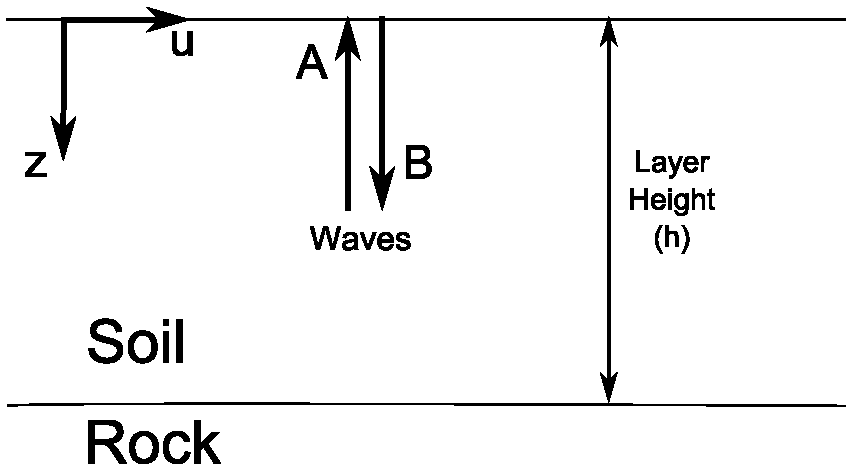
\includegraphics[width=0.7\linewidth]{figures/siteResponse/simpleWave.pdf}
  \end{center}
  \caption{The notation used in the wave equation}
  \label{fig:siteResponse:simpleWave}
\end{figure}

Equation~\ref{eq:waveEq} applies only to a single layer with uniform soil properties and the
wave amplitudes ($A$ and $B$) can be computed from the layer boundary conditions.  For a layered
system, shown in Figure~\ref{fig:siteResponse:nomenclature}, the wave amplitudes are calculated using
recursive formulas developed by maintaining compatibility of displacement and shear stress at the
layer boundaries.  Using these assumptions, the following recursive formulas are developed
\citep{kramer:96}:
\begin{equation}
  \begin{array}{rcl}
	A_{m+1} & = & \frac{1}{2} A_m \left( 1 + \alpha_m^* \right) \exp\left(\imath k_m^* h_m \right) +
	\frac{1}{2} B_m \left( 1 - \alpha_m^* \right) \exp\left(-\imath k_m^* h_m \right)\\
	B_{m+1} & = & \frac{1}{2} A_m \left( 1 - \alpha_m^* \right) \exp\left(\imath k_m^* h_m\right) +
	\frac{1}{2} B_m \left( 1 + \alpha_m^* \right) \exp\left(-\imath k_m^* h_m \right)\\
  \end{array}
\end{equation}
where $m$ is the layer number, $h_m$ is the layer height and $\alpha_m^*$ is the complex impedance
ratio.  The complex impedance ratio is defined as:
\begin{equation}
  \alpha_m^* = \frac{k_m^* G_m^*}{k_{m+1}^* G_{m+1}^*} = \frac{\rho_m v_{s,m}^* }{\rho_{m+1}
  v_{s,m+1}^* } 
\end{equation}
and quantifies the relative amplitudes of the upward and downward waves.  At the surface of the soil
column ($m=1$), the shear stress must equal zero, therefore the amplitudes of the upward and
downward waves must be equal ($A_1=B_1$).  

\begin{figure}
  \begin{center}
	\setlength{\unitlength}{0.6cm}
	\begin{picture}(12,9)
	  % Layers
	  \put(0,1){\line(1,0){12}}
	  \put(0,3){\line(1,0){12}}
	  \put(0,4){\line(1,0){12}}
	  \put(0,5){\line(1,0){12}}
	  \put(0,7){\line(1,0){12}}
	  \put(0,8){\line(1,0){12}}
	  \put(0,9){\line(1,0){12}}
	  % Wave Vectors
	  \thicklines
	  \put(3.9,1){\vector(0,-1){0.75}}
	  \put(3.9,4){\vector(0,-1){0.75}}
	  \put(3.9,5){\vector(0,-1){0.75}}
	  \put(3.9,8){\vector(0,-1){0.75}}
	  \put(3.9,9){\vector(0,-1){0.75}}
	  \put(3.4,0.25){\vector(0,1){0.75}}
	  \put(3.4,3.25){\vector(0,1){0.75}}
	  \put(3.4,4.25){\vector(0,1){0.75}}
	  \put(3.4,7.25){\vector(0,1){0.75}}
	  \put(3.4,8.25){\vector(0,1){0.75}}
	  \put(2.2,8.3){$A_1$}
	  \put(2.2,7.3){$A_2$}
	  \put(2.2,4.3){$A_m$}
	  \put(1.9,3.3){$A_{m+1}$}
	  \put(2.2,0.3){$A_n$}
	  \put(4.1,8.3){$B_1$}
	  \put(4.1,7.3){$B_2$}
	  \put(4.1,4.3){$B_m$}
	  \put(4.1,3.3){$B_{m+1}$}
	  \put(4.1,0.3){$B_n$}

	  % Layer indicators
	  \put(0.0,8.3){$1$}
	  \put(0.0,7.3){$2$}
	  \put(0.0,4.3){$m$}
	  \put(0.0,3.3){$m+1$}
	  \put(0.0,0.3){$n$}
	  % Layer properties
	  \put(6,8.3){\(\rho_{1} \  h_{1} \  G_{1} \  D_{1} \)}
	  \put(6,7.3){\(\rho_{2} \  h_{2} \  G_{2} \  D_{2} \)}
	  \put(6,4.3){\(\rho_{m} \  h_{m} \  G_{m} \  D_{m} \)}
	  \put(6,3.3){\(\rho_{{m+1}} \  h_{{m+1}} \  G_{{m+1}} \  D_{{m+1}} \)}
	  \put(6,0.3){\(\rho_{n} \  h_{n} \  G_{n} \  D_{n} \)}
	\end{picture}
  \end{center}
  \caption{Nomenclature for the theoretical wave propagation.}
  \label{fig:siteResponse:nomenclature}
\end{figure}

The wave amplitudes ($A$ and $B$) within the soil profile are calculated at each frequency (assuming
known stiffness and damping within each layer) and used to computed the response at the surface of a
site.  This calculation is performed by setting $A_{1}=B_{1}=1.0$ at the surface and recursively
calculating the wave amplitudes ($A_{m+1}$,$B_{m+1}$) in successive layers until the input (base)
layer is reached.  The transfer function between the motion in the layer of interest ($m$) and in
the rock layer ($n$) at the base of the deposit is defined as:
\begin{equation}
  TF_{m,n}(\omega) = \frac{u_m(\omega)}{u_n(\omega)}= \frac{A_m + B_m}{A_n + B_n}
  \label{eq:transFunc}
\end{equation}
where $\omega$ is the frequency of the harmonic wave.  The transfer function is the ratio of the
amplitude of motion--either displacement, velocity, or acceleration--between two layers of interest
and varies with frequency.  The transfer function for the site with the properties presented in
Table~\ref{tab:siteResponse:site} is shown in Figure~\ref{fig:siteResponse:transFunc}.  The locations of the
peaks in the transfer function are controlled by the modes of vibration of the soil deposit.  The
peak at the lowest frequency represents the fundamental (i.e. first) mode of vibration and results
in the largest amplification.  The peaks at higher frequencies are the higher vibrational modes of
the site.  The first natural frequency of a site is inversely related to the site period, where the
site period is defined as \citep{kramer:96}:
\begin{equation}
  T_s = \frac{4\cdot h_{soil}}{\overline{v}_s}\\ 
  \label{eq:sitePeriod}
\end{equation}
In equation (\ref{eq:sitePeriod}), $h_{soil}$ is the total height of the soil and $\overline{v}_s$
average velocity of the site.  
% FIXME Insert discussion regarding time averaged vs and fix name of vs

\begin{equation}
	2+2=4
  \label{eq:avgVs}
\end{equation}

For the example site (Table~\ref{tab:siteResponse:site}), the site period is calculated to be 0.57 s
which corresponds to a natural frequency of 1.75 Hz.  In the transfer function
(Figure~\ref{fig:siteResponse:transFunc}), the peak with the highest amplification occurs
at this frequency.  The amplitudes of the peaks are controlled by the damping ratio of the soil. As
the damping of the system increases, the amplitudes of the peaks decrease, which results in less
amplification at the surface.

\begin{table}[t]
  \centering
  \begin{tabular}{llc}
	\hline\hline
	\textbf{Property} & \textbf{Rock} & \textbf{Soil} \\
	\hline
	Mass Density ($\rho$) 		& 2.24 g/cm\textsuperscript{3} & 1.93 g/cm\textsuperscript{3} \\
	Height ($h$)				& $\inf$		& 50 m \\
	Shear-wave Velocity ($v_s$)	& 1500 m/s		& 350 m/s \\
	Damping ratio ($D$)			& 1\%			& 7\% \\
	\hline
  \end{tabular}
  \caption{The site properties of an example site.}
  \label{tab:siteResponse:site}
\end{table}
\begin{figure}[t]
  \begin{center}
	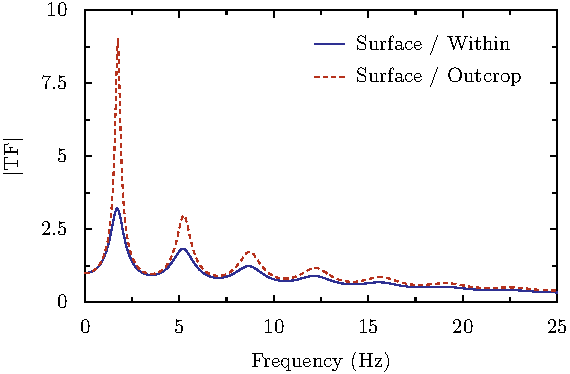
\includegraphics[width=\linewidth]{figures/siteResponse/sra-transFunc.pdf}
  \end{center}
  \caption{The input to surface transfer functions site in Table~\ref{tab:siteResponse:site}
  considering different types of input.}
  \label{fig:siteResponse:transFunc}
\end{figure}


The response at the layer of interested is computed by multiplying the Fourier amplitude spectrum of the
input rock motion by the transfer function\index{transfer function!acceleration}:
\begin{equation}
  Y_m(\omega) = TF_{m,n}(\omega) \cdot Y_n(\omega)
  \label{eq:tfApplication}
\end{equation}
where $Y_n$ is the input Fourier amplitude spectrum at layer $n$ and $Y_m$ is the Fourier amplitude
spectrum at the top of the layer of interest.  The Fourier amplitude spectrum of the input motion
can be defined using a variety of methods and is discussed further in Sections
\ref{ch:siteResponse:methods:timeSeries} and \ref{ch:siteResponse:methods:rvt}.

One issue that must be considered is that the input Fourier spectrum typically represents a motion
at the ground surface, where the upgoing and downgoing wave amplitudes are equal ($A_1=B_1$), not at
the base of a soil deposit, where the wave amplitudes are not equal
(Figure~\ref{fig:siteResponse:outcropWithin}). The change in boundary conditions ( $A_n = B_n$ for
the surface, $A_n \ne B_n$ at the base of a soil deposit) must be taken into account.  The motions
at any free surface are referred to as \emph{outcrop}\index{motion type!outcrop} motions and their
amplitudes are described by twice the amplitude of the upward wave ($2A$).  Equation
(\ref{eq:transFunc}) can be modified to transfer an outcrop motion to a surface motion.  This result
is obtained by multiplying equation (\ref{eq:transFunc}) by a transfer function that takes the
outcrop motions and makes it a within motion at the base of the soil column.

to an \emph{outcrop} motion a second transfer function is required to translate
from an \emph{outcrop} motion to a \emph{within} motion.  The combined transfer function is defined
as:
\begin{equation}
  TF_{m,n}(\omega) = \underbrace{\frac{A_n + B_n}{2\cdot A_n}}_{outcrop \to within} \cdot
  \underbrace{\frac{A_m + B_m}{A_n + B_n}}_{within \to layer_n} = \underbrace{\frac{A_m + B_m}{ 2
  \cdot A_n }}_{outcrop \to layer_n}
  \label{eq:transFunc:withinToOutcrop}
\end{equation}

Motions recorded at depth (e.g. recorded in a borehole) are referred to as
\emph{within}\index{motion type!within} motions and for these motions the transfer function given in
equation (\ref{eq:transFunc}) can be used.  

Figure~\ref{fig:siteResponse:transFunc} shows the transfer function for the site profile presented
in Table~\ref{tab:siteResponse:site} using equation (\ref{eq:transFunc:withinToOutcrop} where the
input motion is specified as \emph{outcrop}. In comparison with the \emph{within}-to-\emph{outcrop}
transfer function, the \emph{outcrop}-to-\emph{outcrop} transfer function displays less
amplification for all modes.

\begin{figure}[tb]
  \begin{center}
	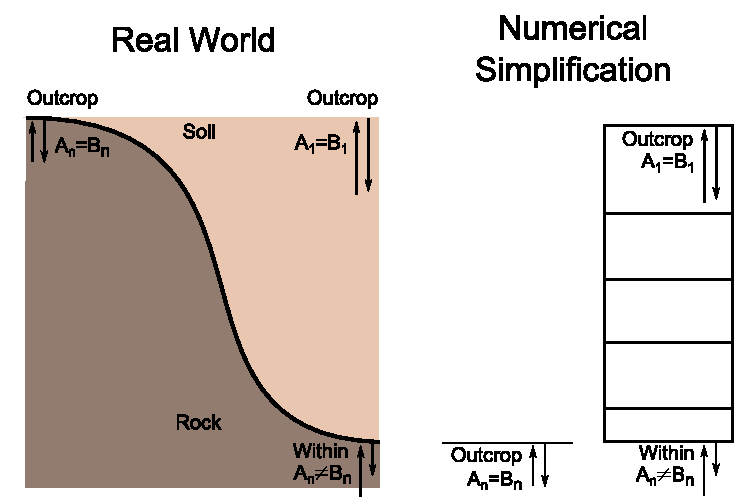
\includegraphics[width=0.7\linewidth]{figures/siteResponse/withinOutcrop.pdf}
  \end{center}
  \caption{\emph{Outcrop} describes upward and downward waves being equal, \emph{within} is used
  when the upward and downward waves are not equal.}
  \label{fig:siteResponse:outcropWithin}
\end{figure}
\clearpage

\subsection{Equivalent-Linear Analysis}\label{ch:siteResponse:equivLinear}
The previous section assumed that the soil was linear-elastic. However, soil is nonlinear, such that
the dynamic properties of soil (shear modulus, $G$, and damping ratio, $D$) vary with shear strain, and
thus the intensity of shaking.  In equivalent-linear site response analysis, the nonlinear response
of the soil is approximated by modifying the linear elastic properties of the soil based on the
induced strain level.  Because the induced strains depend on the soil properties, the strain
compatible shear modulus and damping ratio values are iteratively calculated based on the computed
strain.  

A transfer function is used to compute the shear strain in the layer based on the outcropping input
motion.  In the calculation of the strain transfer function, the shear strain is computed at the middle of
the layer ($z=h_m/2$) and used to select the strain compatible soil properties.  Unlike the previous
transfer functions that merely amplified the Fourier amplitude spectrum, the strain transfer
function\index{transfer function!strain} amplifies the motion and converts acceleration into strain.
The strain transfer function based on an outcropping input motion is defined by:
\begin{equation}
  TF_{mn}^{strain}(\omega) = \frac{\gamma(\omega, z=h_m/2)}{\ddot{u}_{n,outcrop}(\omega)} =
  \frac{\imath k_m \left[
  A_m \exp\left( \imath k_m^* h_m / 2 \right) - B_m \exp\left( -\imath k_m^* h_m / 2 \right) \right]
  }{-\omega^2 \left( 2 \cdot A_n \right)}
  \label{eq:strain_tf}
\end{equation}
The strain Fourier amplitude spectrum within a layer is calculated by applying the strain transfer
function to the Fourier amplitude spectrum of the input motion.  The maximum strain within the layer
is derived from this Fourier amplitude spectrum -- either through conversion to the time domain or
through RVT methods, further discussed in Section~\ref{ch:siteResponse:methods}).  However, it is
not appropriate to use the maximum strain within the layer to compute the strain-compatible soil
properties, because the maximum strain only occurs for an instant in time.  Instead, an effective
strain ($\gamma_{\mathrm{eff}}$) is calculated from the maximum strain.  Typically, the effective
strain is 65\% of the maximum strain. An example of a strain time-series and the effective strain is
shown in Figure~\ref{fig:siteResponse:strainTH}.

% FIXME label the effective strain in the plot
\begin{figure}[tb]
  \begin{center}
	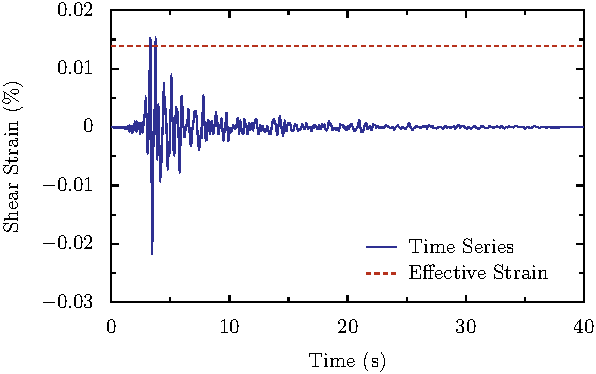
\includegraphics[width=\linewidth]{figures/siteResponse/sra-strain-ts.pdf}
  \end{center}
  \caption{An example of the strain-time history and effective strain ($\gamma_{\mathrm{eff}}$).}
  \label{fig:siteResponse:strainTH}
\end{figure}

Equivalent-linear site response analysis requires that the strain dependent nonlinear properties
(i.e. $G$ and $D$) be defined.  The initial (small strain) shear modulus\index{shear
modulus!maximum (small strain)} ($G_{max}$) is calculated by:
\begin{equation}
  G_{max} = \rho v_s ^ 2
\end{equation}
where $\rho$ is the mass density of the site, and $v_s$ is the measured shear-wave velocity.
Characterizing the nonlinear behavior of $G$ and $D$ is achieved through modulus reduction and
damping curves that describe the variation of $G/G_{max}$ and $D$ with shear strain (discussed in
the next section).  Using the initial dynamic properties of the soil, equivalent-linear site
response analysis involves the following steps:
\begin{enumerate}
  \item The wave amplitudes ($A$ and $B$) are computed for each of the layers
  \item The strain transfer function is calculated for each of the layers.
  \item The maximum strain within each layer is computed by applying the strain transfer function
	to the input Fourier amplitude spectrum and finding the maximum response (see
	Section~\ref{ch:siteResponse:methods}).
  \item The effective strain ($\gamma_{\mathrm{eff}}$) is calculated from the maximum strain within
	each layer.
  \item The strain compatible shear modulus and damping ratio are recalculated based on the new
	estimate of the effective strain within each layer.
  \item The new nonlinear properties ($G$ and $D$) are compared to the previous iteration and an
	error is calculated.  If the error for all layers is below a defined threshold the calculation
	stops.
\end{enumerate}
After the iterative portion of the program finishes, the dynamic response of the soil deposit is
computed.  


% FIXME Find a place to discuss response spectrum

% One method of looking at the response of the soil deposit is with a acceleration response
% spectrum\index{response spectrum}, a tool used in structural analysis to assess the frequency
% content of the response.  An acceleration response spectrum is defined as the maximum accelerations
% of single-degree-of-freedom oscillators with a range of natural periods and a specific damping
% ratio.  The acceleration response spectrum transfer function is defined as:
% \begin{equation}
%   H(f) = \frac{-f_n^2}{(f^2-f_n^2) - 2 \cdot \imath \cdot \xi \cdot f_n \cdot f}
% \end{equation}
% where $f_n$ is the natural frequency of the oscillator, $\xi$ is the damping ratio, and $f$ is the
% frequency. The damping ratio is typically defined at 5\% as this corresponds to the approximate
% damping of an undamaged building.  The response at single period is calculated by applying the
% transfer function to the Fourier spectrum of interest and computing the maximum response.  The
% response spectrum is computed by varying the natural frequency of the oscillator over a range of
% interest, typically 0.01 to 10 seconds.
% 
% \begin{figure}[tb]
%   \begin{center}
% 	\includegraphics[width=\linewidth]{figures/siteResponse/accelSa.pdf}
%   \end{center}
%   \caption{The input and surface acceleration response spectrum ($\xi$=5\%).}
%   \label{fig:siteResponse:accelSa}
% \end{figure}

\subsection{Dynamic Soil Properties}\label{ch:siteResponse:dynprops}
In a dynamic system,  the properties that govern the response are the mass, stiffness, and damping.
In soil under seismic shear loading, the mass of the system is characterized by the mass density
($\rho$) and the layer height ($h$), the stiffness is characterized by the shear modulus ($G$), and
the damping is characterized by the viscous damping ratio ($D$).  The dynamic behavior of soil is
challenging to model because it is nonlinear, such that, both the stiffness and damping of the
system change with shear strain.  Section~\ref{ch:siteResponse:equivLinear} introduced
equivalent-linear site response analysis in which the nonlinear response of the soil was simplified
into a linear system that used strain-compatible dynamic properties ($G$ and $D$).  The analysis
requires that the strain dependence of the nonlinear properties within a layer be fully
characterized.

Defining the mass density of the system is a straight forward process because the density of soil falls
within a limited range for soil and a good estimate of the mass density can be made based on soil
type alone.  Characterization of the stiffness and damping properties of soil is more complicated,
the most rigorous approach requiring testing in both the field and laboratory.  

The shear modulus and material damping of the soil are characterized using the small strain shear
modulus ($G_{max}$), modulus reduction curves that relate $G/G_{max}$ to shear strain, and damping
ratio curves that relate $D$ to shear strain.  The small strain shear modulus is best
characterized by in situ measurement of the shear-wave velocity as a function of depth.  An example
shear-wave velocity profile is shown in Figure~\ref{fig:siteResponse:vsProfile}. The profile tends to be
separated into discrete layers with a generally increasing shear-wave velocity with increasing
depth.  Examples of modulus reduction and damping curves for soil are shown in
Figure~\ref{fig:siteResponse:nlLab}.  These curves show a decrease in the soil stiffness and an
increase in the damping ratio with an increase in shear strain. 

\begin{figure}[tb]
  \begin{center}
	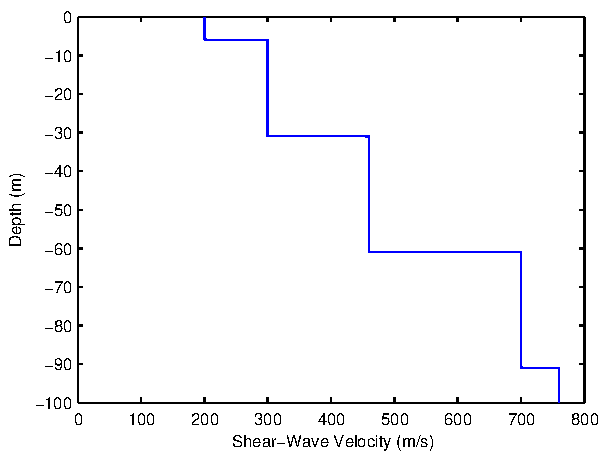
\includegraphics{figures/siteResponse/vsProfile.pdf}
  \end{center}
  \caption{An example shear-wave velocity profile}
  \label{fig:siteResponse:vsProfile}
\end{figure}
\begin{figure}[tb]
  \centering
  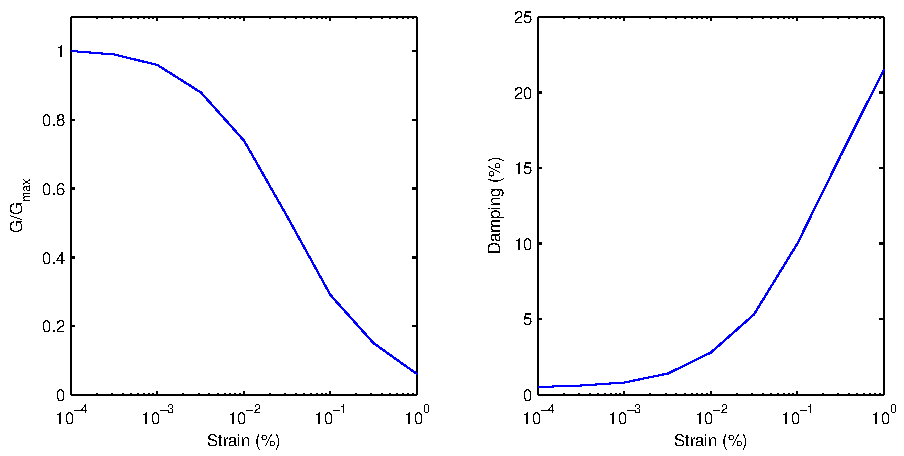
\includegraphics[width=\textwidth]{figures/siteResponse/nlLab.pdf}
  \caption{Examples of shear modulus reduction and material damping curves for soil.}
  \label{fig:siteResponse:nlLab}
\end{figure}

The modulus reduction and damping curves may be obtained from laboratory measurements on soil
samples or derived from empirical models based on soil type and other variables.  One of the most
comprehensive empirical models was developed by \citet{darendeli:01} and is included with Strata.
The model expands on the hyperbolic model presented by \citet{hardin:72} and accounts for the
effects of confining pressure ($\sigma_0'$), plasticity index ($PI$), over-consolidation ratio
($OCR$), frequency ($f$), and number of cycles of loading ($N$) on the modulus reduction and damping
curves. 

In the \citet{darendeli:01} model, the shear modulus reduction curve is a hyperbola defined by:
\begin{equation}
  \frac{G}{G_{max}} = \frac{1}{1 + \left( \frac{\gamma}{\gamma_r} \right)^{a}}
  \label{eq:shearmod}
\end{equation}
where $a$ is 0.9190, $\gamma$ is the shear strain and $\gamma_r$ is the reference shear strain.  The reference
shear strain (not in percent) is computed from:
\begin{equation}
  \gamma_r = \left(\frac{\sigma_0'}{p_a}\right)^{0.3483} \left( 0.0352 + 0.0010 \cdot PI \cdot OCR^{0.3246} \right)
\end{equation}
where $\sigma_0'$ is the mean effective stress and $p_a$ is the atmospheric pressure in atm. In the
model, the damping ratio is calculated from the minimum damping ratio at small strains ($D_{min}$)
and from the damping ratio associated with hysteretic Masing behavior ($D_{Masing}$).  The minimum
damping is calculated from:
\begin{equation}
  D_{min}(\%) = (\sigma_0')^{-0.2889} \left( 0.8005 + 0.0129 \cdot PI \cdot OCR ^{-0.1069} \right) \left[
  1 + 0.2919 \ln\left( f \right) \right]
  \label{eq:dmin}
\end{equation}
where $f$ is the excitation frequency (Hz). The computation of the Masing damping requires the
calculation of the area within the stress-strain curve predicted by the shear modulus reduction
curve.  The integration can be approximated by:
\begin{equation}
  D_\text{Masing}(\%) = c_1 D_{\text{Masing},a=1} + c_2 D_{\text{Masing},a=1}^2 + c_3
  D_{\text{Masing},a=1}^2
  \label{eq:dmasing}
\end{equation}
where:
\begin{equation}
  D_{masing,a=1}(\%) = \frac{100}{\pi} \left\{ 4 \left[ \frac{\gamma - \gamma_r\ln\left( \frac{\gamma +
  \gamma_r}{\gamma_r} \right)}{\frac{\gamma^2}{\gamma+\gamma_r}} \right] - 2 \right\} \\
\end{equation}
\begin{equation}
  \begin{array}{rcl}
	c_1 & = & -1.1143 a^2 + 1.8618 a + 0.2533 \\
	c_2 & = & 0.0805 a^2 - 0.0710 a - 0.0095 \\
	c_3 & = & -0.0005 a^2 + 0.0002 a + 0.0003 \\
  \end{array}
\end{equation}
The minimum damping ratio in equation (\ref{eq:dmin}) and the Masing damping in equation
(\ref{eq:dmasing}) are combined to compute the total damping ratio ($D$) using:
\begin{equation}
  D = b  \left( \frac{G}{G_{max}} \right)^{0.1} \cdot D_{Masing} + D_{min} 
  \label{eq:damping}
\end{equation}
where $b$ is defined as:
\begin{equation}
  b = 0.6329 - 0.0057 \ln\left( N \right)
\end{equation}
where $N$ is the number of cycles of loading.  In most site response applications, the number of
cycles ($N$) and the excitation frequency ($f$) in the model are defined as 10 and 1,
respectively.  Figure~\ref{fig:siteResponse:nlEmpirical} shows the predicted nonlinear curves for a sand
($PI=0, OCR=1$) at an effective confining pressure of 1 atm.

\begin{figure}[tb]
  \begin{center}
	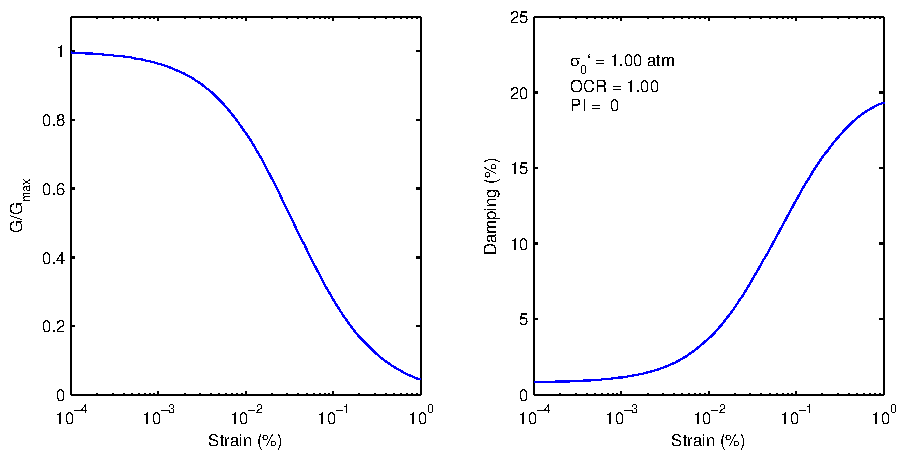
\includegraphics[width=\linewidth]{figures/siteResponse/nlEmpirical.pdf}
  \end{center}
  \caption{The nonlinear soil properties predicted by the \citet{darendeli:01} model.}
  \label{fig:siteResponse:nlEmpirical}
\end{figure}

A Bayesian approach was used in the \citet{darendeli:01} model to calculate the model coefficients.
One of the unique aspects of this model is that the scatter of the data about the mean estimate is
quantified.  In the \citet{darendeli:01} model, the variability about the mean value is assumed to
be normally distributed.  The normal distribution is described using a mean and standard deviation.
The mean values are calculated from equations (\ref{eq:shearmod}) and (\ref{eq:damping}). The
standard deviation is a function of the amplitude of the nonlinear property (i.e. $G/G_{max}$ and
$D$).  The standard deviation of the normalized shear modulus ($\sigma_{NG}$) is computed by:
\begin{equation}
  \sigma_{NG} = \exp(-4.23) + \sqrt{ \frac{0.25}{\exp(3.62)} - \frac{\left(G/G_{max} -
  0.5\right)^2}{\exp(3.62)} }
  \label{eq:sigmaShear}
\end{equation}
This model results in small $\sigma_{NG}$ when $G/G_{max}$ is close to 1 or 0 and relatively large
$\sigma_{NG}$ when $G/G_{max}$ is equal to 0.5. The standard deviation of the damping ratio
($\sigma_{D}$) is computed by:
\begin{equation}
  \sigma_{D} = \exp(-5.0) + \exp(-0.25) \sqrt{D (\%)}
  \label{eq:sigmaDamping}
\end{equation}
In the damping ratio model, the $\sigma_{D}$ increases with increasing damping ratio.  Using these
definitions for the standard deviation, the $\pm\sigma$ modulus reduction and damping curve for sand
at a confining pressure of 1 atm are shown in Figure~\ref{fig:siteResponse:nlEmpiricalSigma}.

\begin{figure}[tb]
  \begin{center}
	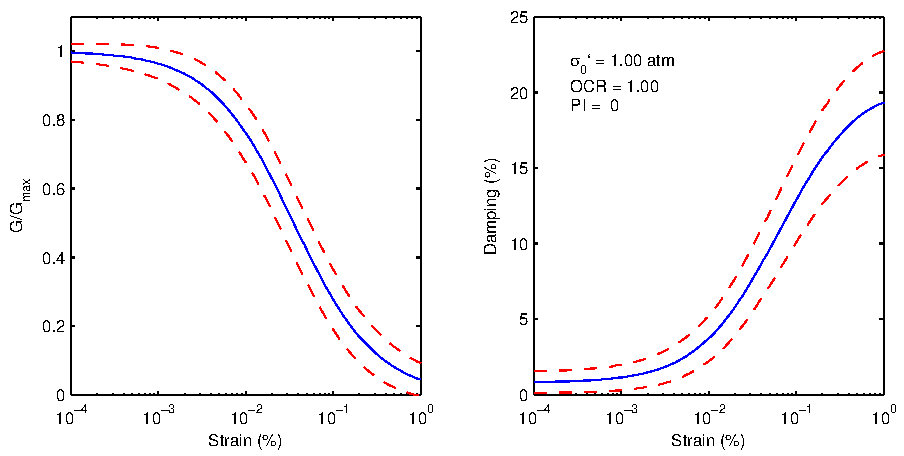
\includegraphics[width=\linewidth]{figures/siteResponse/nlEmpiricalSigma.pdf}
  \end{center}
  \caption{The mean and mean $\pm\sigma$ nonlinear soil properties predicted by \citet{darendeli:01}.}
  \label{fig:siteResponse:nlEmpiricalSigma}
\end{figure}
\clearpage 

\section{Site Response Methods}\label{ch:siteResponse:methods}
The previous section introduced transfer functions which transform the input Fourier amplitude
spectrum (FAS) into a FAS of strain, acceleration, and even a single-degree-of-freedom oscillator at
any depth within the site profile.  In both the time domain and random vibration theory methods, the
same transfer functions are applied to the input FAS.  The difference in the methods is in how this
FAS in the frequency domain is converted into the time domain information.

\subsection{Time Series Method}\label{ch:siteResponse:methods:timeSeries}
In the time series method, an input acceleration-time history is provided and the input FAS is
computed from that time series using the fast Fourier transform (FFT)\index{fast Fourier transform}
to compute the discrete Fourier transformation on the provided
time series.  The computed FAS is complex valued, and can be converted into amplitude and phase
information.  Strata uses the free and open-source FFTW library (\texttt{http://www.fftw.org}).
The inverse discrete Fourier transform is used to compute a time series for a given FAS.  The
details of the FFT process are not discussed here, but can be found on the FFTW webpage.

In Strata, the time series is padded with zeros to obtain a number of points that is a power of two.
If a time series contains a power of two values, then it is padded with zeros until the next power
of two.

The frequencies associated with the FAS are computed from the time step between points and the
number of points ($N$) in the record.  The highest possible sampling frequency is known as the
Nyquist frequency\index{Nyquist frequency} and is defined as:
\begin{equation}
  f_{Nyquist} = \frac{1}{2 \Delta t}
\end{equation}
where $\Delta t$ is the time increment between data points.  The increment between the frequencies
is calculated by:
\begin{equation}
  \Delta f = \frac{f_{Nyquist}}{N/2-1} = \frac{1}{ 2 \Delta t \left( N/2 - 1 \right)}
\end{equation}

After the FAS of the motion has been computed it is possible to perform site response
analysis with the motion.  The following is a summary of the steps to compute the surface
acceleration time-series for the site described in Table~\ref{tab:siteResponse:site}:
\begin{enumerate}
  \item Read the acceleration-time series file (Figure~\ref{fig:siteResponse:timeDomainSequence}a).
  \item Compute the input FAS with the Fast Fourier transformation (FFT)
	(Figure~\ref{fig:siteResponse:timeDomainSequence}b, only amplitude is shown).
  \item Compute the transfer function for the site properties
	(Figure~\ref{fig:siteResponse:timeDomainSequence}c, only amplitude is shown).
  \item Compute the surface FAS by applying the transfer function to the input FAS
	(Figure~\ref{fig:siteResponse:timeDomainSequence}d, only amplitude is shown).
  \item Compute the surface acceleration-time series through the inverse FFT of the surface FAS
	(Figure~\ref{fig:siteResponse:timeDomainSequence}e).
\end{enumerate}

\begin{figure}[p]
  \begin{center}
	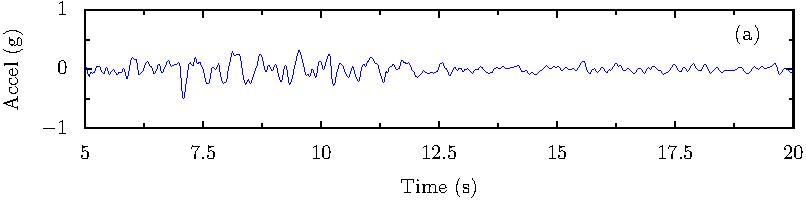
\includegraphics[width=0.95\linewidth]{figures/siteResponse/td-rock-accel-ts.pdf}
	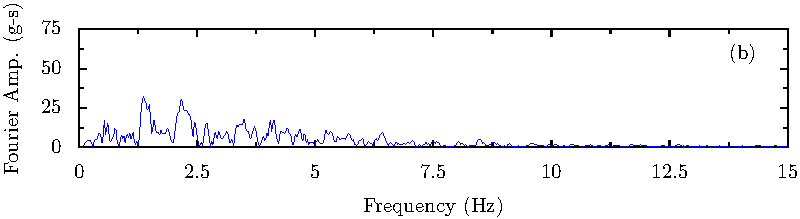
\includegraphics[width=0.95\linewidth]{figures/siteResponse/td-rock-fas.pdf}
	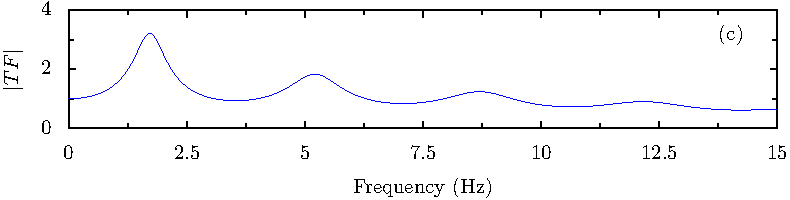
\includegraphics[width=0.95\linewidth]{figures/siteResponse/td-rock-surface-tf.pdf}
	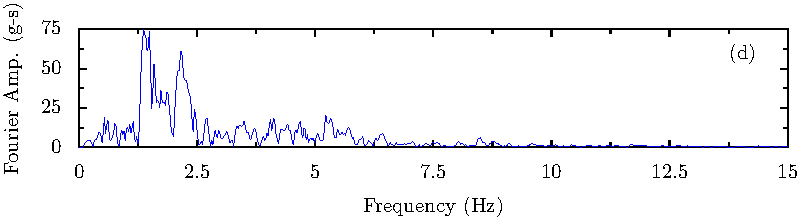
\includegraphics[width=0.95\linewidth]{figures/siteResponse/td-surface-fas.pdf}
	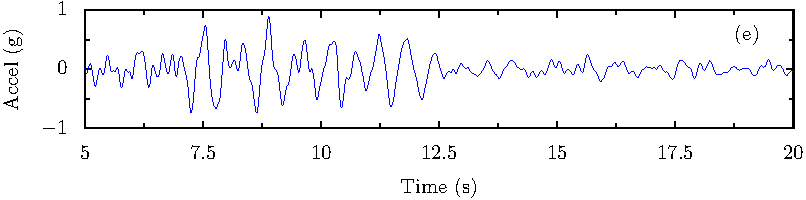
\includegraphics[width=0.95\linewidth]{figures/siteResponse/td-surface-accel-ts.pdf}
  \end{center}
  \caption[Time domain method sequence]{Time domain method sequence: (a) input acceleration-time series, (b) input
  Fourier amplitude spectrum, (c) transfer function from input to surface, (d) surface Fourier
  amplitude spectrum, and (e) surface acceleration-time series.}
  \label{fig:siteResponse:timeDomainSequence}
\end{figure}

\subsection{Random Vibration Theory Method}\label{ch:siteResponse:methods:rvt}
The random vibration theory (RVT) approach to site response analysis was first proposed in the
engineering seismology literature (e.g. ~\citet{schneider:91}) and has been applied to site response
analysis \citep{silva:97,rathje:05}. RVT does not utilize time domain input motions, but rather
initiates all computtions with the input FAS (amplitude only, no phase information).  Because RVT
does not have the accompanying phase angles to the Fourier amplitudes, a time history of motion
cannot be computed.  Instead, extreme value statistics are used to compute peak time domain
parameters of motion (e.g. peak ground acceleration, spectral acceleration) from the Fourier
amplitude information. Due to RVT's stochastic nature one analysis can provide a median estimate of
the site response with a single analysis and with the need for time domain input motions.  

\subsubsection{The Basics of RVT}
Random vibration theory can be separated into two parts: (1) conversion between time and frequency
domain using Parseval's theorem, and (2) estimation of the peak factor using extreme value
statistics.

Consider a time varying signal $x(t)$ with its associated Fourier amplitude spectrum, $X(f)$.  The
root-mean-squared value of the signal ($x_{rms}$) is a measure of its average value over a given
time period, $T_{rms}$, and is computed from the integral of the times series over that time period:
\begin{equation}
  x_{rms} = \sqrt{ \frac{1}{T_{rms}} \int_0^{T_{rms}} \left[ x(t) \right]^2 \ud t }
  \label{eq:a_rms}
\end{equation}
Parseval's theorem\index{random vibration theory!Parseval's theorem} related the integral of the time series to the integral of its Fourier Transform,
such that Equation~\ref{eq:a_rms} can be written in term of the FAS of the signal:
\begin{equation}
  x_{rms} = \sqrt{ \frac{2}{T_{rms}} \int_0^{\infty} |X(f)|^2 \ud f } = \sqrt{\frac{m_0}{T_{rms}}}
  \label{eq:rvt:rms}
\end{equation}
where $m_0$ is defined as the zero-th moment of the FAS.  The $n$-th moment of the FAS is defined
as:
\begin{equation}
  m_n = 2 \int_0^{\infty} \left( 2 \pi f \right)^n |X(f)|^2 \ud f
  \label{eq:rvt:moments}
\end{equation}

The peak factor ($PF$) represents the ratio of the maximum value of the signal ($x_{max}$) to its
$rms$ value ($x_{rms}$), such that if $x_{rms}$ and $PF$ are known, then $x_{max}$ can be computed
using:
\begin{equation}
  x_{max} = PF \cdot x_{rms}
  \label{eq:rvt:max}
  \index{random vibration theory!peak factor}
\end{equation}
\citet{cartwright:56} studied the statistics of ocean wave amplitudes, and considered the
probability distribution of the maxima of a signal to develop expressions for the $PF$ in terms of
the characteristics of the signal.  \citet{cartwright:56} derived an integral expression for the
expected values of the peak factor in terms of the number of extrema ($N_e$) and the bandwidth
($\xi$) of the time series \citep{boore:03}:
\begin{equation}
  E[PF] = \sqrt{2} \int_0^{\infty} 1 - \left[ 1 - \xi\exp\left( -z^2 \right) \right]^{N_e} \ud z
  \label{eq:rvt:peakFactor}
\end{equation}
where the bandwidth is defined as:
\begin{equation}
  \xi = \sqrt{\frac{m_2^2}{m_0 m_4}}
  \label{eq:rvt:bandWidth}
\end{equation}
and the number of extrema is defined as:
\begin{equation}
  N_e = \frac{1}{\pi} \sqrt{\frac{m_4}{m_2}} T_{gm}
  \label{eq:rvt:numExtrema}
\end{equation}

\citet{boore:84} illustrated the need to modify the duration used in the \emph{rms} calculation when
considering oscillator responses, and they introduced the concept of an \emph{rms} duration
($T_{rms}$).  The \emph{rms} duration requires modification for spectral acceleration to account for
the enhanced duration due to the oscillator response.  Generally, adding the oscillator duration to
the ground motion duration will suffice, except in cases where the ground motion duration is
short~\citep{boore:84}.  \citet{boore:84} recommend the following expressions to define $T_{rms}$:
\begin{equation}
  T_{rms} = T_{gm} + T_o \left( \frac{\gamma^n}{\gamma^n + \alpha} \right)
  \label{eq:durationRms}
\end{equation}
\begin{equation}
  \gamma = \frac{T_{gm}}{T_n}
\end{equation}
\begin{equation}
  T_o = \frac{T_n}{2\pi\beta}
\end{equation}
where $T_o$ is the oscillator duration, $T_n$ is the oscillator natural period, and $\beta$ is the
damping ratio of the oscillator.  Based on numerical simulations, \citet{boore:84} proposed $n=3$
and $\alpha=\frac{1}{3}$ for the coefficients in Equation~\ref{eq:durationRms}.

\subsubsection{Defining the Input Motion}
% FIXME Source theory has been added
The input motion in an RVT analysis is defined by a ground motion duration ($T_{gm}$) and a Fourier
amplitude spectrum (FAS).  The FAS can be directly computed using seismological source theory (e.g
\citep[e.g.][]{brune:70,brune:71}), or it can be back-calculated from an acceleration response
spectrum (see section~\ref{ch:siteResponse:methods:rvt:inversion} on
page~\pageref{ch:siteResponse:methods:rvt:inversion}).  Strata does not provide implementation for
any seismological source theory models but does allow for the Fourier amplitude spectrum to be
directly provided.  The frequencies provided with the Fourier amplitude spectrum is the frequency
range used by the program so it is critical that enough points be provided.

Calculation of the duration for use in RVT analysis can be done using seismological source theory or
empirical models.  \citet{boore:03} recommends the following description of ground motion duration
($T_{gm}$) for the Western United States:
\begin{equation}
  T_{gm} =  \underbrace{\frac{1}{f_0}}_\text{Source duration, $T_s$} + \underbrace{0.05
  R}_\text{Path duration, $T_p$}
\end{equation}
where $R$ is the distance in km, and the corner frequency ($f_o$) in hertz is given by:
\begin{displaymath}
	f_0 = 4.9 \cdot 10^6 \beta_s \left( \frac{\Delta\sigma}{M_0} \right)^{1/3} 
\end{displaymath}
where $\Delta\sigma$ is the stress drop in bar, $\beta_s$ is the shear-wave velocity in units of
km/s, and $M_0$ is the seismic moment is units of dyne-cm \citep{brune:70,brune:71}.  The seismic
moment ($M_0$) is related to the moment magnitude ($M_w$) by:
\begin{displaymath}
	M_0 = 10^{\frac{3}{2}\left( M_0 + 10.7 \right)}
\end{displaymath}
For the Eastern United States, \citet{campbell:03} proposes that the path duration effect be
distance dependent:
\begin{equation}
  T_p = \left\{
  \begin{array}{ll}
	0 & R \le 10 \text{km} \\
	0.16R & 10 \text{km} < R \le 70 \text{km} \\
	-0.03R & 70 \text{km} < R \le 130 \text{km} \\
	0.04R & R > 130 \text{km} \\
  \end{array}
  \right.
\end{equation}
Empirical ground motions duration models \citep[e.g.][]{abrahamson:96} can also be used to estimate the duration of the scenario
event ($T_{gm}$).  When such a model is applied, it is recommended that $T_{gm}$ be taken as time
between the build up from 5\% to 75\% of the normalized arias intensity ($D_{5-75}$).

% FIXME provide Abrahamson and Silva 1996?

\subsubsection{Calculation of a FAS from an Acceleration Response
Spectrum}\label{ch:siteResponse:methods:rvt:inversion}\index{random vibration theory!response
spectrum inversion}

The input rock FAS ($Y(f)$) can be derived from an acceleration response spectrum using an inverse
technique.  The inversion technique follows the basic methodology proposed by \citet{gasparini:76} and further
described by \citet{rathje:05}.  The inversion technique makes use of the properties of the
single-degree-of-freedom (SDOF) transfer function used to compute the response spectral values.
The square of the Fourier amplitude at the SDOF oscillator natural frequency
$f_n$ ($|Y(f_n)|^2$) can be written in terms of the spectral acceleration at $f_n$ ($S_{a,f_n}$),
the peak factor ($PF$), \emph{rms} duration of the motion ($T_{rms}$), the square of the Fourier
amplitudes ($|Y(f)|^2$) at frequencies less than the natural frequency, and the integral of the SDOF
transfer function ($|H_{f_n}(f)|^2$):
\begin{equation}
  |Y(f_n)|^2 \approx  \frac{1}{\int_{0}^{\infty} |H_{f_n}(f)|^2 \ud f - f_n} \left(
  \frac{T_{rms}}{2}\frac{S_{a,f_n}^2}{PF^2} - \int_{0}^{f_n} |Y(f)|^2 \ud f
  \right)
  \label{eq:irvt:complex}
\end{equation}
Within Equation~\ref{eq:irvt:complex}, the integral of the transfer function is constant for a given
natural frequency and damping ratio ($\beta$), allowing the equation to be simplified to \citep{gasparini:76}:
\begin{equation}
  |Y(f_n)|^2 \approx  \frac{1}{f_n \left( \frac{\pi}{4\beta} - 1 \right)} \left(
  \frac{T_{rms}}{2}\frac{S_{a,f_n}^2}{PF^2} - \int_{0}^{f_n} |Y(f)|^2 \ud f
  \right)
  \label{eq:irvt:simple}
\end{equation}

The peak factors in Equation~\ref{eq:irvt:simple} depend on the moments of the FAS which is
currently undefined.  So the peak factors for all natural frequencies are initially assumed to be 2.5.
Equation~\ref{eq:irvt:simple} is applied first to the spectral acceleration of the lowest frequency
(longest period) provided by the user. At this frequency, the FAS integral term in Equation~\ref{eq:irvt:simple}
can be assumed to be equal to zero.  The equation is then applied at successively higher frequencies
using the previously computed values of $|Y(f)|$ to assess the integral.

After an initial estimate of the FAS is developed using Equation~\ref{eq:irvt:simple} with assumed
constant peak factors, it would be possible to recompute the peak factors for each period.  The
variable peak factors would provide a better estimate of the FAS from the target response spectrum.
This approach was originally implemented, but the FAS based on the variable peak factors still
resulted in a response spectrum that was more than 10\% different than the target response spectrum
at short periods.

To improve the agreement between the RVT-derived FAS (and associated response spectrum) and the
target response spectrum by correcting the FAS by the ratio of the two response spectra.  This
correction technique is possible because of the narrow band property of the SDOF transfer function.
Using an iterative process, the FAS from iteration $i$ is corrected by the ratio of the spectral
acceleration computed by RVT ($S_{a}^{\text{RVT}}(f)$) to the target
($S_{a}^{\text{target}}(f)$) at each frequency:
\begin{equation}
  |Y_{i+1}(f)| = \frac{S_{a}^{\text{RVT}}(f)}{S_{a}^{\text{target}}(f)} |Y_{i+1}(f)|
  \label{eq:saRatioCorrection}
\end{equation}
The following process is used in the generate a corrected FAS:
\begin{enumerate}
  \item Initial FAS is computed using the \citet{vanmarcke:83} technique.
  \item The acceleration response spectrum associated with this FAS is computed using RVT.
  \item The FAS is corrected using equation (\ref{eq:saRatioCorrection}).
  \item Using the corrected FAS, a new acceleration response spectrum is calculated.
\end{enumerate}
This process is repeated with three conditions:
\begin{enumerate}
  \item maximum of 30 iterations,
  \item a root-mean-square-error of 0.005 is achieved, or
  \item the change in the root-mean-square-error is less than 0.001.
\end{enumerate}
This ratio correction works very well in producing a FAS that agrees with the target response
spectrum, but the resulting FAS may have an inappropriate shape at some frequencies, as discussed
below.

To demonstrate the inversion process consider a scenario event of a magnitude 6.5 earthquake with a
strike-slip faulting mechanism at a distance of 20 km.  The target response spectrum is computed
using the \citet{abrahamson:97} attenuation model (Figure~\ref{fig:irvt:sa}).  An initial estimate
of the FAS is computed using the \citet{gasparini:76} method and then the ratio correction algorithm
is applied.  This methodology results in a good agreement -- less than 5\% relative error as shown
in Figure~\ref{fig:irvt:error} -- with the target response spectrum (Figure~\ref{fig:irvt:sa}), but
the associated FAS tends to curl up at low and high frequencies (curve labeled ``Ratio Corrected''
in Figure~\ref{fig:irvt:fas}).  The curling up at low frequencies can be mitigated by extending the
frequency domain.  

The frequency domain is extended to half of the minimum frequency and twice the maximum
frequency specified in the target response spectrum.  For example, if the target response spectrum is provided from 0.2 to 100 Hz (5
to 0.01 seconds), then the frequencies of the FAS are defined to be 2048 points equally spaced in log
space from  0.1 to 200 Hz.  The resulting response spectrum shows even better agreement with a
maximum error of about 3\% (curve labeled ``Ratio and Extrapolated'' in Figure~\ref{fig:irvt:error}).  

% FIXME Rathje wants to talk about th
Theoretically the slope of the FAS at high frequencies should be increasingly negative due to a
path-independent loss of the high-frequency motion \citep{boore:03}.  However, in the computed
FAS the slope actually increases at around 50 Hz (Figure~\ref{fig:irvt:fas}).  At first glance it
may not appear that this relatively small amount of high frequency energy is important.  However, in
site response analysis the damping in the soil further attenuates this high frequency portion of the
FAS, and the peak factor depends on the 4\textsuperscript{th} moment which is sensitive to this high
frequency energy.  The result is that the strain (or acceleration) near the surface -- after
attenuation of the high frequency energy has occurred -- is significantly less than it computed
using traditional time domain methods.  To solve for this shortcoming, the slope of the FAS at high
frequencies is forced down (Figure~\ref{fig:irvt:fas}).  However, this solution results in a slight under
prediction of the peak ground acceleration (Figure~\ref{fig:irvt:sa} and \ref{fig:irvt:error}).

\begin{figure}[p]
  \begin{center}
	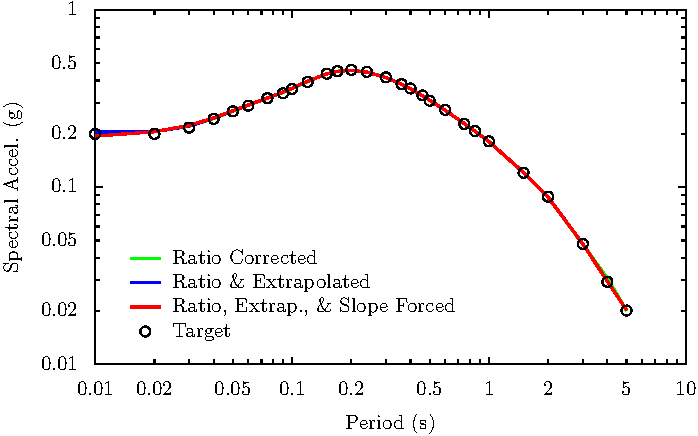
\includegraphics[width=0.95\linewidth]{figures/siteResponse/irvt-respSpec.pdf}
  \end{center}
  \caption{The comparison between the target response spectrum and the response spectrum computed with
  RVT.}
  \label{fig:irvt:sa}
\end{figure}
\begin{figure}[p]
  \begin{center}
	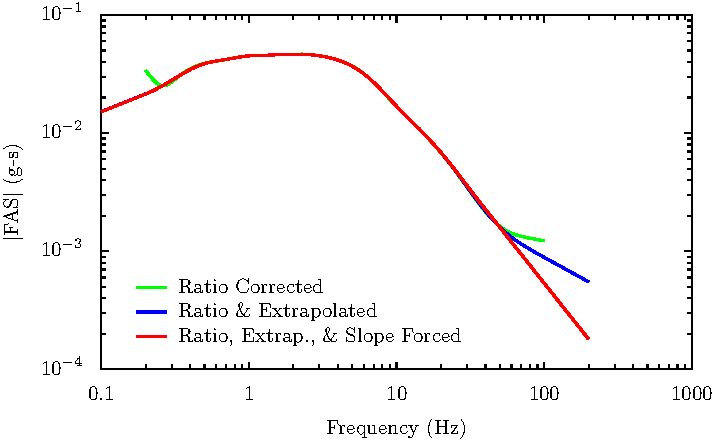
\includegraphics[width=0.95\linewidth]{figures/siteResponse/irvt-fas.pdf}
  \end{center}
  \caption{The FAS computing through the inversion process.}
  \label{fig:irvt:fas}
\end{figure}
\begin{figure}[tb]
  \begin{center}
	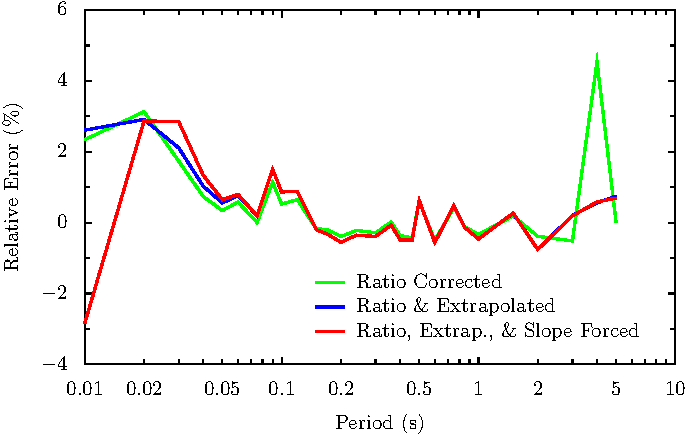
\includegraphics[width=\linewidth]{figures/siteResponse/irvt-error.pdf}
  \end{center}
  \caption{The relative error between the computed response spectra and the target response spectrum.}
  \label{fig:irvt:error}
\end{figure}

\clearpage
\subsubsection{Example of the RVT Procedure}
The following is an example of the random vibration theory based site response analysis to estimate
the peak acceleration at the top of the site described in Table~\ref{tab:siteResponse:site}:  The
earthquake scenario is a magnitude 6.5 event at a distance of 20 km, as described in the previous
section.
\begin{enumerate}
  \item Empirical relationships are used to specify the input rock response spectrum
	  (Figure~\ref{fig:irvt:sa}) and ground motion duration ($T_{gm}=D_{5-75}=$4.55s).
  \item Using the inversion technique, the FAS corresponding to the target response spectrum is
	computed (Figure~\ref{fig:siteResponse:rvtSequence}a). In this example, the maximum acceleration
	of the input motion is computed with RVT to allow for a comparison in the peak response between the surface and the
	input.  The RVT calculation results are shown in Table~\ref{tab:rvtSequence:input}.

	\begin{table}[h]
	  \centering
	  \begin{tabular}{l r @{.} l l}
		\hline\hline
		\textbf{Parameter} & \multicolumn{2}{c}{\textbf{Input Motion Value}} & \textbf{Equation} \\
		\hline
		Moments of FAS ($m_0$, $m_2$, and $m_4$) & 0&0280, & \ref{eq:rvt:moments} \\
		& 93&8435, and \\
		& 1&7382 $\cdot 10^7$  \\
		Bandwidth ($\xi$) & 0&1346 & \ref{eq:rvt:bandWidth} \\
		Number of extrema ($N_e$) & 623&3158 & \ref{eq:rvt:numExtrema} \\
		Peak factor ($PF$) & 3&1406 & \ref{eq:rvt:peakFactor} \\
		Root-mean-square acceleration ($a_{rms}$) & 0&0784 g & \ref{eq:rvt:rms} \\
		\\
		Expected maximum acceleration ($a_{max}$) & 0&2462 g & \ref{eq:rvt:max} \\
		\hline\hline
	  \end{tabular}
	  \caption{The values of the RVT calculation for the input motion.}
	  \label{tab:rvtSequence:input}
	\end{table}

  \item Compute the transfer function for the site properties
	(Figure~\ref{fig:siteResponse:rvtSequence}b).
  \item Compute the surface FAS by applying the absolute value of the transfer function to the input
	  FAS (Figure~\ref{fig:siteResponse:rvtSequence}c).  Using the surface FAS the maximum expected
	  acceleration can be computed as presented in Table~\ref{tab:rvtSequence:surface}.  The
	  calculation shows that the site response increases the expected peak ground acceleration by
	  approximately 34\%.

	\begin{sidewaystable}[h]
	  \centering
	  \begin{tabular}{l r @{.} l  r @{.} l l}
		\hline\hline
		& \multicolumn{4}{c}{\textbf{Value}}  \\
		\textbf{Parameter} & \multicolumn{2}{c}{\textbf{Input Motion}} &
		\multicolumn{2}{c}{\textbf{Surface Motion}} & \textbf{Equation} \\
		\hline
		Moments of FAS ($m_0$, $m_2$, and $m_4$) & 0&0280, & 0&0635, & \ref{eq:rvt:moments} \\
		& 93&8435, and & 39&6356, and \\
		& 1&7382 $\cdot 10^7$ & 1&6306 $\cdot 10^5$  \\
		Bandwidth ($\xi$) & 0&1346 & 0&3895 & \ref{eq:rvt:bandWidth} \\
		Number of extrema ($N_e$) & 623&3158 & 92&8944 & \ref{eq:rvt:numExtrema} \\
		Peak factor ($PF$) & 3&1406 & 2&8568 & \ref{eq:rvt:peakFactor} \\
		Root-mean-square acceleration ($a_{rms}$) & 0&0784 g & 0&1181 g & \ref{eq:rvt:rms} \\
		\\
		Expected maximum acceleration ($a_{max}$) & 0&2462 g & 0&3375 g & \ref{eq:rvt:max} \\
		\hline\hline
	  \end{tabular}
	  \caption{The values of the RVT calculation for the input and surface motions.}
	  \label{tab:rvtSequence:surface}
	\end{sidewaystable}

\end{enumerate}

\begin{figure}[p]
  \begin{center}
	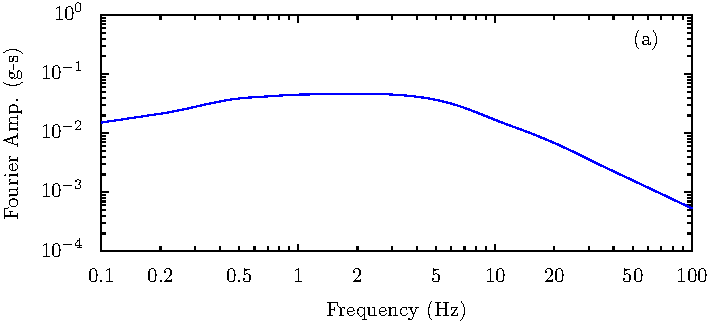
\includegraphics[width=0.95\linewidth]{figures/siteResponse/rvt-rock-fas.pdf}
	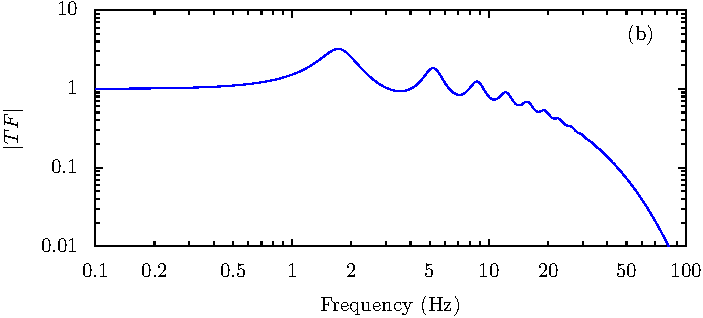
\includegraphics[width=0.95\linewidth]{figures/siteResponse/rvt-rock-surface-tf.pdf}
	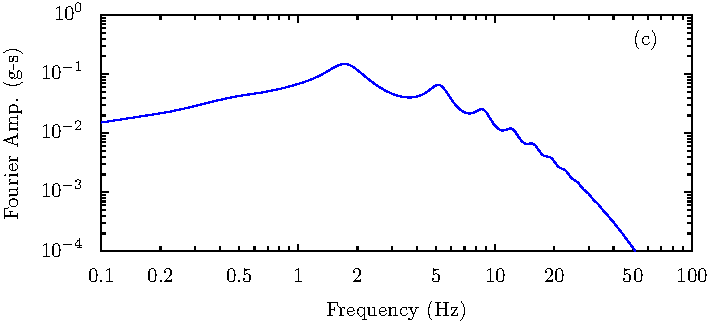
\includegraphics[width=0.95\linewidth]{figures/siteResponse/rvt-surface-fas.pdf}
  \end{center}
  \caption[RVT method sequence]{Random vibration theory method sequence: (a) input
  Fourier amplitude spectrum, (b) transfer function from input to surface, and (c) surface Fourier
  amplitude spectrum.}
  \label{fig:siteResponse:rvtSequence}
\end{figure}

\chapter{Variation of Site Properties}\label{ch:var}
\section{Introduction}
A soil profile consists of discrete layers that vary in thickness based on the properties of the
soil.  The layers are typically discretized based on the soil type, recorded from borehole samples
or inferred from a shear-wave velocity profile. In seismic site response analysis, each layer is
characterized by a thickness, mass density, shear-wave velocity, and nonlinear properties
($G/G_{max}$, and $D$).  One of the challenges in defining values for these properties is the
natural variability across a site and the uncertainty in their measurement.  Because the dynamic response of
a site is dependent on the soil properties, any variation in the soil properties will change both
the expected surface motion and its standard deviation.

In a simple system, the variability of the components can be analytically combined to quantify the
variability of the complete system, thus allowing for the expected value and variability of the
system response to be computed. In seismic site response analysis, the nonlinear response of the
system does not allow an exact analytic quantification of the variability of the site response.
Instead, an estimate of the expected surface response and its standard deviation due to variations
in the soil properties can be made through Monte Carlo simulations.  Monte Carlo simulations
estimate the response of a system by generating parameters of the system based on defined
statistical distributions and computing the response for each set of input parameters.  The
following chapter introduces Monte Carlo simulations as applied to site response analysis and
presents the models that describe the variability of the layering, shear-wave velocity, and
nonlinear properties ($G/G_{max}$ and $D$).  

\section{Random Variables}
The goal of a Monte Carlo simulation is to estimate the statistical properties of the response of a
complex system.  To achieve this goal, each of the properties of the system is selected from defined
statistical distributions and the response of the system is computed.  The response is computed for
many realizations and the calculated response from each realization is then used to estimate
statistical properties of the system's response. While Monte Carlo simulations can be used on a wide
variety of problems, a major disadvantage is that a large number of simulations is required to
achieve stable results.

Monte Carlo simulations require that each of the components in the system has a complete statistical
description.  The description can be in the form of a variety of statistical distributions (i.e.
uniform, triangular, normal, log-normal, exponential, etc.), however the normal and log-normal
distributions typically are used because they can be easily described using a mean ($\mu$) and
standard deviation ($\sigma$).  For normally distributed variables, a random value ($x$) can be
generated by:
\begin{equation}
  x = \sigma_x \cdot \varepsilon + \mu_x
  \label{eq:randVar}
\end{equation}
where $\mu_x$ is the mean value, $\sigma_x$ is the standard deviation, and $\varepsilon$ is a random
variable with zero mean and unit standard deviation.  

There are a variety of methods for generating random variables for a given distribution.  The most
general technique involves using the cumulative density function (CDF) to convert between
probability and value.  For example, the calculation of a normally distributed random variable is
achieved by first calculating a random variable from a uniform distribution between 0 and 1.  The
random variable ($\varepsilon$) is then calculated by finding the inverse to this random value on
the standard ($\sigma$=1) normal CDF, shown in Figure~\ref{fig:rand:variable}.  If the distribution
of the variable is not normal, a similar technique of using a random value from a unit uniform
distribution and the CDF of the probability distribution of the variable can be used
\citep{ang:vol2}.  While this method is applicable for a set of independent random variables, it may
not be used when the variables are related (i.e. correlated).

\begin{figure}[tb]
  \begin{center}
	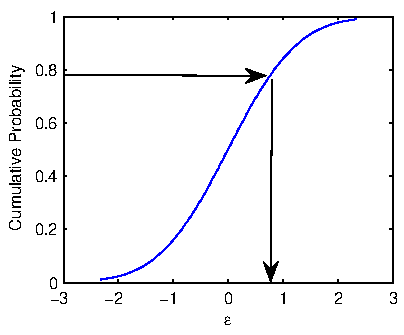
\includegraphics{figures/rand/variable.pdf}
  \end{center}
  \caption{Using a random variable from a uniform distribution between 0 and 1 to generate a
  variable from a distribution with a zero mean and unit standard deviation.}
  \label{fig:rand:variable}
\end{figure}

%FIXME Add something regarding random number generation

In the case of random variables that are not independent, a more complicated procedure is required
for the generation of values. Before discussing the technique for generating correlated random
variables, the concepts of correlation and linear functions of random variables must be introduced. 

Consider random variables $x_1$ and $x_2$.  The covariance of the two random variables is defined as:
\begin{equation}
  \textrm{cov}(x_1, x_2) = E[(x_1 - \mu_{x_1})(x_2 - \mu_{x_2})] = E[x_1 x_2] - E[x_1] E[x_2]
\end{equation}
where $E$ is the expected value and $\mu_{x_1}$ and $\mu_{x_2}$ are the mean values of $x_1$ and
$x_2$, respectively \citep{ang:vol1}.  The covariance quantifies the strength of relationship between
$x_1$ and $x_2$. If the variables are independent of each other (Figure~\ref{fig:rand:correl}a),
then the covariance is zero, however a covariance of zero does not necessarily indicate the
variables are independent. Instead, it indicates that the variables do not have a linear dependence.
As the covariance becomes more positive, two variables have a greater tendency to both differ from
their respective mean values in the same direction (Figure~\ref{fig:rand:correl}b).  Conversely, as
the covariance becomes more negative, variables have a greater tendency to differ in the opposite
direction ( Figure~\ref{fig:rand:correl}c).  The covariance matrix ($[C]$) of a set of random
variables is defined as:
\begin{equation}
  [C]_{i,j}  = \mathrm{cov}(X_i,X_j)
  \label{eq:covMatrix}
\end{equation}

For two variables, the covariance matrix expands to:
\begin{equation}
  [C] = 
  \left[
  \begin{array}{cc}
	\textrm{cov}(x_1, x_1) & \textrm{cov}(x_1, x_2 ) \\
	\textrm{cov}(x_2, x_1) & \textrm{cov}(x_2, x_2 ) \\
  \end{array}
  \right]
  = 
  \left[
  \begin{array}{cc}
	\sigma_{x_1} ^ 2 & \rho_{x_1, x_2} \sigma_{x_1} \sigma_{x_2} \\
	\rho_{x_1, x_2} \sigma_{x_1} \sigma_{x_2} & \sigma_{x_2} ^ 2 \\
  \end{array}
  \right]
\end{equation}
where $\sigma_{x_1}$ and $\sigma_{x_2}$ are the standard deviations of $x_1$ and $x_2$,
respectively, and $\rho_{x_1, x_2}$ is the correlation coefficient, defined as:
\begin{equation}
  \rho_{x_1,x_2} = \frac{\mathrm{cov}(x_1,x_2)}{\sigma_{x_1} \sigma_{x_2}} = 
  \frac{E[x_1 x_2] - E[x_1] E[x_2]}{\sigma_{x_1} \sigma_{x_2}}
  \label{eq:correlCoeff}
\end{equation}
The correlation coefficient can range -1 to 1.

\begin{figure}[tb]
  \begin{center}
	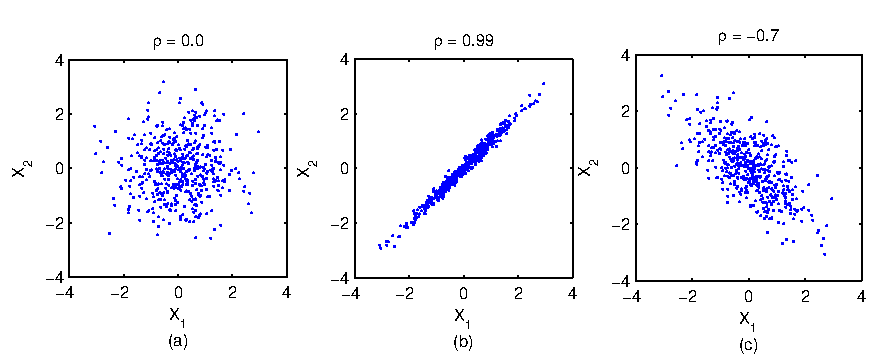
\includegraphics[width=\textwidth]{figures/rand/correlation.pdf}
  \end{center}
  \caption{Two variables with a correlation coefficient of: (a) 0.0, (b), 0.99, and (c) -0.7.}
  \label{fig:rand:correl}
\end{figure}

Independent random variables from a normal distribution are generated using equation
(\ref{eq:randVar}) independently for each random variable. By combining the multiple applications
equation (\ref{eq:randVar}) into a system of equations, the generation of two independent variables
is achieved by multiplying a vector of random variables ($\vec{\varepsilon}$) by a matrix
($[\sigma]$) and adding a constant ($\vec{\mu}$), defined as:
\begin{equation}
  \left\{
  \begin{array}{c}
	x_1 \\
	x_2 \\
  \end{array}
  \right\} 
  =
  \left[
  \begin{array}{ccc}
	\sigma_{x_1} & 0 \\
	0 & \sigma_{x_2} \\
  \end{array}
  \right]
  \left\{
  \begin{array}{c}
	\varepsilon_1 \\
	\varepsilon_2 \\
  \end{array}
  \right\}
  + 
  \left\{
  \begin{array}{c}
	\mu_1 \\
	\mu_2 \\
  \end{array}
  \right\}
  \label{eq:linearSystem:uncorrel}
\end{equation}
where $\varepsilon_1$ and $\varepsilon_2$ are random variables randomly selected from a standard
normal distribution ($\mu=0$ and $\sigma=1$), $\sigma_{x_1}$ and $\sigma_{x_2}$ are the standard
deviations of $x_1$ and $x_2$, respectively, and $\mu_{x_1}$ and $\mu_{x_2}$ are the mean values of
$x_1$ and $x_2$, respectively.  Because the random variables $x_1$ and $x_2$ are independent
($\rho_{x_1,x_2}=0$), the off-diagonal values in the matrix ($[\sigma]$) are zero.  

Using the same framework, a linear system of equations is used to generate a pair of correlated
random variables.  However, because of the correlation between $x_1$ and $x_2$ the off diagonal
values in the matrix will no longer be zero.  Instead, a pair of correlated random variables
($\vec{x}$) are generated by:
\begin{equation}
  \left\{
  \begin{array}{c}
	x_1 \\
	x_2 \\
  \end{array}
  \right\} 
  =
  \left[
  \begin{array}{cc}
	\sigma_{x_1} & 0 \\
	\rho_{x_1,x_2}\sigma_{x_2} & \sigma_{x_2} \sqrt{1 - \rho_{x_1,x_2}^2} \\ 
  \end{array}
  \right]
  \left\{
  \begin{array}{c}
	\varepsilon_1 \\
	\varepsilon_2 \\
  \end{array}
  \right\}
  + 
  \left\{
  \begin{array}{c}
	\mu_1 \\
	\mu_2 \\
  \end{array}
  \right\}
  \label{eq:linearSystem:correlSol}
\end{equation} % FIXME reference for this?
Here, the first random variable ($x_1$) is calculated based on the value of $\varepsilon_1$ alone,
while the second random variable ($x_2$) is a function of both $\varepsilon_1$ and $\varepsilon_2$.
Note that $\varepsilon_1$ and $\varepsilon_2$ still represent random and independent variables
generated from the standard normal distribution.

\section{Statistical Models for Soil Properties}
For the properties of the soil to be randomized and incorporated into Monte Carlo simulations, the
statistical distribution and properties of the soil need to be characterized.  In this research, two
separate models are used.  The first model, developed by \citet{toro:95}, describes the statistical
distribution and correlation between layering and shear-wave velocity.  The second model by
\citet{darendeli:01} was previously introduced in Section~\ref{ch:siteResponse:dynprops} and is used to
describe the statistical distribution of the nonlinear properties ($G/G_{max}$ and $D$).

\subsection{Layering and Velocity Model}\label{ch:var:models:layering}
In Strata, the randomization of the layering and the shear-wave velocity is done through the
use of the velocity profile model proposed by \citet{toro:95}.  The \citet{toro:95} models provides
a framework for generating layering and then to vary the shear-wave velocity of these layers.   This model
improves upon previous work by quantifying the correlation between the velocities in adjacent
layers.  In previous models, one of two assumptions were made that simplified the problem: the
velocities at all depths were perfectly correlated and could be randomized by applying a constant
random factor to all velocities \citep{mcguire:89, toro:92}, or the velocities within each of the
layers are independent of each other, and therefore can be randomized by applying an independent
random factor to each layer \citep{costantino:91}. While these two assumptions simplify the problem,
they represent two extreme conditions.  The \citet{toro:95} model makes neither of these
assumptions, instead the model incorporates a correlation between layers.

\subsubsection{Layering Model}
The layering is modeled as a Poisson process, which is a stochastic process with events occuring at
a given rate ($\lambda$).  For a homogeneous Poisson process this rate is constant, while for a
non-homogeneous Poisson process the rate varies.  Generally, a Poisson process models the occurrence
of events over time, but for the layering problem the event is a layer interface and its rate is
defined in terms of length (i.e., number of layer interfaces per meter).

% FIXME Rathje says: ``I think this is confusing because depth and thickness are not the same.  Depth is
% measured from the surface and thickness from the layer above.  Thus, this write is confusing to
% me''.
In the \citet{toro:95} model, the layering thickness is modeled as non-homogeneous Poisson process
where the rate changes with depth ($\lambda(d)$, where $d$ is depth).  Before considering the
non-homogeneous Poisson process, first consider the simpler homogeneous Poisson process with a
constant rate.  For a Poisson process with a constant occurrence rate ($\lambda$), the distance
between layer boundaries, or layer thickness ($h$), is an exponential distribution with rate
$\lambda$.  The probability density function of an exponential distribution is defined as:
\begin{equation}
  f(h;\lambda) = 
  \left\{
  \begin{array}{ll}
	\lambda \exp(-\lambda h) & \text{for } h \ge 0 \\
	0 & \text{for } h < 0 \\
  \end{array}
  \right.
  \label{eq:exponential:pdf}
\end{equation}
The cumulative density function for the exponential distribution is given by:
\begin{equation}
  F(h;\lambda) = 
  \left\{
  \begin{array}{ll}
	1- \exp(-\lambda h) & \text{for } h \ge 0 \\
	0 & \text{for } h < 0 \\
  \end{array}
  \right.
  \label{eq:exponential:cdf}
\end{equation}
A random layer thickness with an exponential distribution is generated by solving
Equation~\ref{eq:exponential:cdf} with respect to thickness ($t$):
\begin{equation}
  h = \frac{\ln\left[1-F(h)\right]}{-\lambda} \quad \text{for } 0 < F(h) \le 1
  \label{eq:exponential:inv}
\end{equation}
By randomly generating probabilities ($F(t)$) with a uniform distribution and computing the
associated thicknesses with Equation~\ref{eq:exponential:inv}, a layering profile was simulated for
8 layers with a rate of 1 shown in Figure~\ref{fig:rand:poisson:homo}.

\begin{figure}[tb]
  \begin{center}
	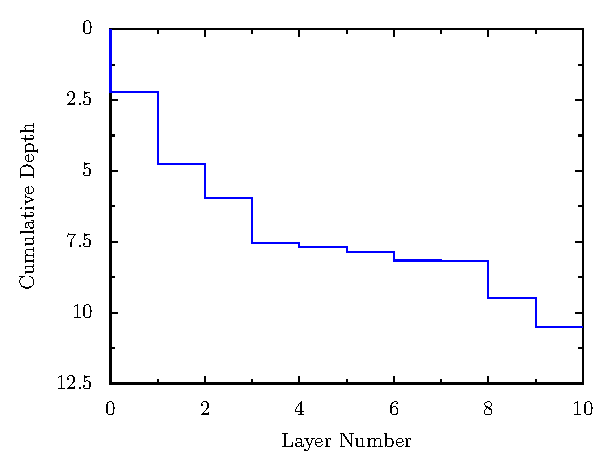
\includegraphics{figures/rand/poisson-homo}
  \end{center}
  \caption{A layering profile consisting of 8 layers modeled by a homogeneous Poisson process with a rate of 1.}
  \label{fig:rand:poisson:homo}
\end{figure}

% FIXME need references for warping 
Simulating a non-homogeneous Poisson process is achieved by first simulating a homogeneous Poisson
process and then warping the homogeneous layer boundaries ($S'_n$) into the non-homogeneous
equivalent ($S_n$).  The process is very similar to the generation of random variables with a
specific distribution where a uniform distribution is warped into a particular distribution using
the CDF.  For a non-homogeneous Poisson process with rate $\lambda(d)$ the cumulative rate
($\Lambda(d)$) is defined as:
\begin{equation}
  \Lambda(d) = \int_{0}^{d} \lambda(s) \ud s
  \label{eq:poisson:cumulativeRate}
\end{equation}
$\Lambda(d)$ represents the expected number of layers up to a depth $d$.  The non-homogeneous
process is simulated by generating exponential distributions with a unit rate ($\lambda=1$) and
mapping them to the non-homogeneous space using the inverse of
Equation~\ref{eq:poisson:cumulativeRate} ($\Lambda^{-1}(d)$).  

As an example, the warping technique
will be used on the homogeneous Poisson process to take a unit rate exponential random variables and
convert them into a non-unit rate





Before $\Lambda^{-1}(d)$ can be
defined, $\Lambda(d)$ and $\lambda(d)$ must be defined.

\citet{toro:95} proposed the following generic depth dependent rate model:
\begin{equation}
  \lambda(d)= a \cdot (d + b)^{c}
  \label{eq:toro:rate:generic}
\end{equation}
The coefficients $a$, $b$, and $c$ were estimated by \citet{toro:95} using the method of maximum
likelihood applied to the layering measured at 557 sites, coming mostly from California.  The
resulting values of $a$ be 1.98, 10.86, and -0.89, respectively.  The occurrence rate ($\lambda(d)$) quickly
decreases as the depth increases (Figure~\ref{fig:rand:toro}(a)).  This decrease in the
occurrence rate increases the expected thickness of deeper layers.  The expected layer thickness
($h$) is equal to the inverse of the occurrence rate ($\lambda(d)$) and is shown in
Figure~\ref{fig:rand:toro}(b).  The expected thickness ranges from 4.2 m at the surface to
59 m at a depth of 200 m.

\begin{figure}[htb]
  \begin{center}
	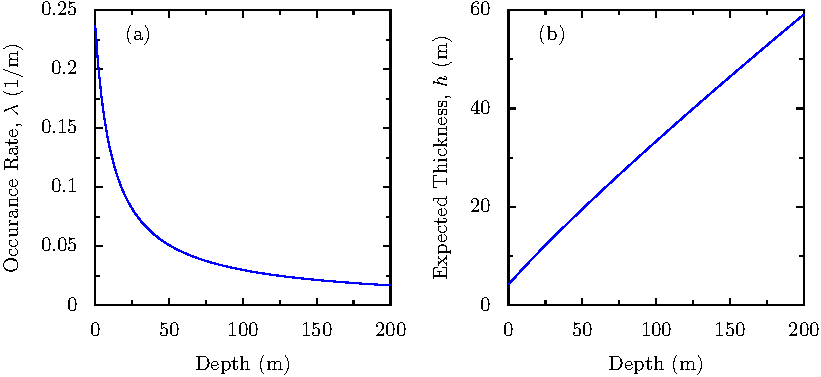
\includegraphics[width=\linewidth]{figures/rand/toro.pdf}
  \end{center}
  \caption{\citet{toro:95} layering model. (a) The occurrence rate ($\lambda$) as a function of depth
  ($d$), and (b) the expected layer thickness ($h$) as a function of depth.}
  \label{fig:rand:toro}
\end{figure}

Using Equations \ref{eq:poisson:cumulativeRate} and \ref{eq:toro:rate:generic} the cumulative rate
for the \citet{toro:95} modeled is defined as:
\begin{equation}
	\Lambda(d) = \int_{0}^{d} a \cdot (s + b)^{c} \ud s = a \cdot \left[\frac{(d+b)^{c+1}}{c+1} -\frac{b^{c+1}}{c+1} \right]
  \label{eq:toro:cumRate}
\end{equation}
The inverse cumulative rate function is then defined as:
\begin{equation}
  \Lambda^{-1}(d)=\left( \frac{c \cdot d}{a} + \frac{d}{a} + b^{c+1} \right)^\frac{1}{c+1} - b 
  \label{eq:toro:invCumRate}
\end{equation}
Using this equation the homogeneous Poisson process (Figure~\ref{fig:rand:poisson:homo}) can
be warped into a non-homogeneous Poisson process as shown in Figure~\ref{fig:rand:poisson:transform}.
The resulting depth profile is shown in Figure~\ref{fig:rand:poisson:nonHomo}.

\begin{figure}[p]
  \begin{center}
	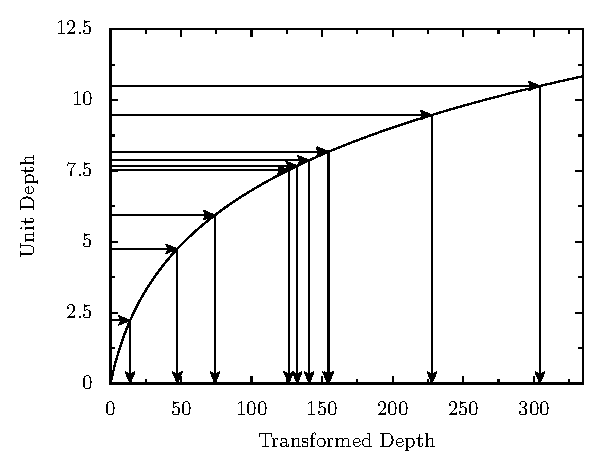
\includegraphics{figures/rand/poisson-warping}
  \end{center}
  \caption{Transformation between a homogeneous Poisson process with rate 1 to the \citet{toro:95}
  non-homogeneous Poisson process.}
  \label{fig:rand:poisson:transform}
\end{figure}
\begin{figure}[p]
  \begin{center}
	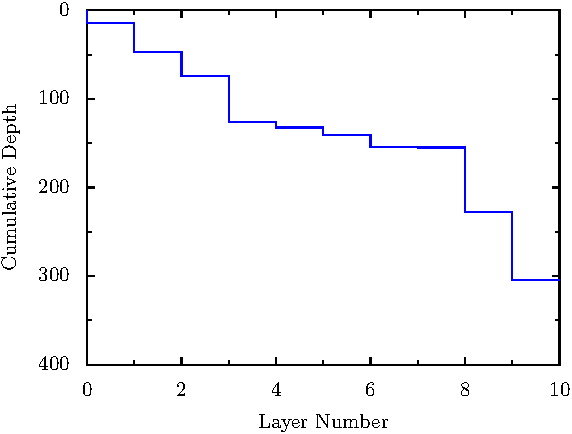
\includegraphics{figures/rand/poisson-nonHomo}
  \end{center}
  \caption{A layering simulated with the non-homogeneous Poisson process defined by
  \citet{toro:95}.}
  \label{fig:rand:poisson:nonHomo}
\end{figure}

\subsubsection{Velocity Model}
%FIXME add discussion of truncation to the model

After the layering of the profile has been established, the shear-wave velocity profile can be
generated.  In the \citet{toro:95} model, the shear-wave velocity at mid-depth of the layer is
described by a log-normal distribution.  The standard normal variable ($Z$) of the $i^{th}$ layer is
calculated by:
\begin{equation}
  Z_i = \frac{\ln(V_i) - \ln[ V_\text{median}(d_i)]}{\sigma_{\ln\ V_s}}
  \label{eq:vsPercentile}
\end{equation}
where $V_i$ is the shear-wave velocity in the $i^{th}$ layer, $V_\text{median}(d_i)$ is the median
shear-wave velocity at mid-depth of the layer and $\sigma_{\ln\ V_s}$ is the standard deviation of the
natural logarithm of the shear-wave velocity.  Equation~\ref{eq:vsPercentile} is then solved for the
shear-wave velocity of the $i^{th}$ layer ($V_i$):
\begin{equation}
  V_i = \exp \left\{ \sigma_{\ln\ V} \cdot Z_i + \ln \left[ V_{median}(d_i) \right] \right\}
  \label{eq:layerVs}
\end{equation}
Equation~\ref{eq:layerVs} allows for the calculation of the velocity within a layer for a given
median velocity at the mid-depth of the layer, standard deviation, and standard normal variable.  In
the model proposed by \citet{toro:95}, values for median velocity versus depth ($V_\text{median}(d)$) and
standard deviation ($\sigma_{\ln\ V_s}$) are provided based on site class. However, in the
implementation of the \citet{toro:95} model in Strata the median shear-wave velocity is defined by
the user.  The standard normal variable of the $i^{th}$ layer ($Z_i$) is correlated with the layer
above it, and this inter-layer correlation is also dependent on the site class.  The standard normal
variable ($Z_i$) of the shear-wave velocity in the top layer ($i=1$) is independent of all other
layers and is defined as:
\begin{equation}
  Z_1 = \varepsilon_1
\end{equation}
where $\varepsilon_1$ is an independent normal random variable with zero mean and a unit standard
deviation.  The standard normal variables of the other layers in the profile are calculated by a
recursive formula, defined as:
\begin{equation}
  Z_i = \rho \cdot Z_{i-1} + \varepsilon_i \cdot \sqrt{1 - \rho^2} \\
\end{equation}
where $Z_{i-1}$ is the standard normal variable of the previous layer, $\varepsilon_i$ is a new
normal random variable with zero mean and unit standard deviation, and $\rho$ is the inter-layer
correlation.  

Correlation is a measure of the strength and direction of a relationship between two random
variables.  The inter-layer correlation between the shear-wave velocities proposed by
\citet{toro:95} is a function of both the depth of the layer ($d$) and the thickness of the layer
($h$):
\begin{equation}
  \rho(d,h) = \left[1 - \rho_d(d)\right] \cdot \rho_h(h) + \rho_d(d)
\end{equation}
where $\rho_h$ is the thickness dependent correlation and $\rho_d$ is the depth dependent
correlation.  The thickness dependent correlation is defined as:
\begin{equation}
  \rho_h(h) = \rho_0 \cdot \exp\left(\frac{-h}{\Delta}\right)
\end{equation}
where $\rho_0$ is the initial correlation and $\Delta$ is a model fitting parameter.  As the
thickness of the layer increases, the thickness-dependent correlation decreases.  The depth
dependent correlation ($\rho_d$) is defined as a function of depth ($d$): 
\begin{equation}
  \rho_d(d) = 
  \left\{
  \begin{array}{ll}
	\rho_{200} \cdot \left[ \frac{d+d_0}{200+d_0} \right]^b & \mathrm{for}\ d \leq 200 \\
	\rho_{200} & \mathrm{for}\ d > 200 \\
  \end{array}
  \right. 
\end{equation}
where $\rho_{200}$ is the correlation coefficient at 200 m and $d_0$ is an initial depth parameter.
As the depth of the layer increases, the depth-dependent correlation increases.  The final layer in
a site response model is assumed to be infinitely thick, therefore the correlation between the last
soil layer and the infinite half-space is only dependent on $\rho_d$.  \citep{toro:95} evaluated
each of the parameters in the correlation models ($\rho_0, \rho_{200}, \Delta, d_0, b$) for
different generic site classes.

A site class is used to categorize a site based on the shear-wave velocity profile and/or local
geology.  In the \citet{toro:95} model, the statistical properties of the soil profile (the median
velocity, standard deviation, and layer correlation) are provided for two different classifications
schemes, the Geomatrix and USGS classifications. The Geomatrix site classification classifies sites
based on a general description of the geotechnical subsurface conditions, distinguishing generally
between rock, shallow soil, deep soil, and soft soil (Table~\ref{tab:rand:geomatrix}).  In contrast,
the USGS site classification is based on the time-weighted average shear-wave velocity (see
equation~\ref{eq:avgVs} of the top 30 meters ($\overline{v}_{s,30}$) (Table~\ref{tab:rand:usgs}),
and requires site specific measurements of shear-wave velocity.

\begin{table}[tbp]
  \centering
  \begin{tabular}{cp{4in}}
	\hline\hline
	\textbf{Designation} & \textbf{Description} \\
	\hline
	\textbf{A}	& Rock \\
	& Instrument is found on rock material ($v_s$ $>$ 600 m/s) or a very thin veneer (less
	than 5 m) of soil overlying rock material.\\
	\\
	\textbf{B}	& Shallow (Stiff) Soil \\
	& Instrument is founded in/on a soil profile up to 20 m thick overlying rock
	material, typically a narrow canyon, near a valley edge, or on a hillside.\\
	\\
	\textbf{C}	& Deep Narrow Soil \\
	& Instrument is found in/on a soil profile at least 20 m thick overlying rock
	material in a narrow canyon or valley no more than several kilometers wide.\\
	\\
	\textbf{D}	& Deep Broad Soil \\
	& Instrument is found in/on a soil profile at least 20 m thick overlaying rock
	material in a broad canyon or valley.\\
	\\
	\textbf{E}	& Soft Deep Soil \\
	& Instrument is found in/on a deep soil profile that exhibits low average shear-wave
	velocity ($v_s$ $<$ 150 m/s).\\
	\hline\hline
  \end{tabular}
  \caption{The categories of the geotechnical subsurface conditions (third letter) in the Geomatrix
  site classification \citep{toro:95}.}
  \label{tab:rand:geomatrix}
\end{table}
\begin{table}[tbp]
  \centering
  \begin{tabular}{cl}
	\hline\hline
	\textbf{Designation} & \textbf{Average Shear-Wave Velocity} ($\overline{v}_{s,30}$)\\
	\hline
	\textbf{A} & greater than 750 m/s \\
	\textbf{B} & 360 to 750 m/s \\
	\textbf{C} & 180 to 360 m/s \\
	\textbf{D} & less than 180 m/s \\
	\hline\hline
  \end{tabular}
  \caption{The USGS site categories, where $\overline{v}_{s,30}$ is the time weighted average
  shear-velocity of the top 30 m \citep{toro:95}.}
  \label{tab:rand:usgs}
\end{table}

\citet{toro:95} computed the statistical properties of the profiles for both the Geomatrix and USGS
classifications using a maximum-likelihood procedure.  The procedure used a total of 557 profiles,
with 541 profiles for the USGS classification and only 164 profiles for the Geomatrix
classification.  The correlation parameters ($\rho_0, \rho_{200}, \Delta, d_0, b$) are presented in
Table~\ref{tab:rand:coeffs} and the median shear-wave velocities in are presented in
Table~\ref{tab:rand:velocity}.

\begin{table}[tbp]
  \centering
  \begin{tabular}{lcc|cccccc}
	\hline\hline
	& \multicolumn{8}{c}{\textbf{Site Classification}} \\
	\hline
	& \multicolumn{2}{c|}{\textbf{GeoMatrix}} 
	& \multicolumn{6}{c}{\textbf{USGS}} \\
	\textbf{Parameter} & A \& B & C \& D & A \& B & C \& D &
	A & B & C & D  \\
	\hline
	$\sigma_{ln V}$	& 0.46 & 0.38 & 0.35 & 0.36 & 0.36 & 0.27 & 0.31 & 0.37 \\
	$\rho_0$ 		& 0.96 & 0.99 & 0.95 & 0.99 & 0.95 & 0.97 & 0.99 & 0.00 \\
	$\rho_{200}$ 	& 0.96 & 1.00 & 1.00 & 1.00 & 0.42 & 1.00 & 0.98 & 0.50 \\
	$\Delta$ 		& 13.1 & 8.0 & 4.2 & 3.9 & 3.4 & 3.8 & 3.9 & 5.0 \\
	$d_0$ 			&  0.0 & 0.0 & 0.0 & 0.0 & 0.0 & 0.0 & 0.0 & 0.0 \\
	$b$ 			& 0.095 & 0.160 & 0.138 & 0.293 & 0.063 & 0.293 & 0.344 & 0.744 \\
	\\
	Profiles 		& 45  & 109 & 204 & 253   & 35  & 169 & 226  & 27 \\
	Layers 			& 243 & 692 & 280 & 1487  & 129 & 750 & 1349 & 136 \\
	\hline\hline
  \end{tabular}
  \caption{Coefficients for the \citet{toro:95} model, calculated by maximum likelihood.}
  \label{tab:rand:coeffs}
\end{table}
\begin{table}[tbp]
  \centering
  \begin{tabular}{ccc|cccccc}
	\hline\hline
	& \multicolumn{8}{c}{\textbf{Median Shear-Wave Velocity (m/s)}} \\
	\hline
	& \multicolumn{2}{c|}{\textbf{GeoMatrix}} 
	& \multicolumn{6}{c}{\textbf{USGS}} \\
	\hline
	\textbf{Depth (m)} & A \& B & C \& D & A \& B & C \& D &
	A & B & C & D  \\
	\hline
	0.00 &  192 & 144 & 182 & 147 &  314 & 159 & 145 & 176 \\
	1.00 &  209 & 159 & 221 & 164 &  346 & 200 & 163 & 165 \\
	2.00 &  230 & 178 & 262 & 178 &  384 & 241 & 179 & 154 \\
	3.00 &  253 & 193 & 297 & 188 &  430 & 275 & 191 & 142 \\
	4.00 &  278 & 204 & 330 & 193 &  485 & 308 & 200 & 129 \\
	5.00 &  303 & 211 & 362 & 196 &  550 & 337 & 208 & 117 \\
	6.00 &  329 & 217 & 390 & 200 &  624 & 361 & 215 & 109 \\
	7.20 &  357 & 228 & 412 & 209 &  703 & 382 & 226 & 106 \\
	8.64 &  395 & 240 & 437 & 218 &  789 & 404 & 237 & 109 \\
	10.37 &  443 & 253 & 468 & 228 &  880 & 433 & 250 & 117 \\
	12.44 &  502 & 270 & 504 & 248 &  973 & 467 & 269 & 130 \\
	14.93 &  575 & 291 & 540 & 273 & 1070 & 501 & 291 & 148 \\
	17.92 &  657 & 319 & 578 & 296 & 1160 & 535 & 314 & 170 \\
	21.50 &  748 & 357 & 615 & 317 & 1260 & 567 & 336 & 192 \\
	25.80 &  825 & 402 & 653 & 347 & 1330 & 605 & 372 & 210 \\
	30.96 &  886 & 444 & 702 & 374 & 1380 & 654 & 391 & 229 \\
	37.15 &  942 & 474 & 734 & 386 & 1420 & 687 & 401 & 246 \\
	44.58 &  998 & 495 & 759 & 394 & 1460 & 711 & 408 & 266 \\
	53.20 & 1060 & 516 & 782 & 403 & 1500 & 732 & 413 & 289 \\
	64.20 &      & 541 & 805 & 427 &      & 749 & 433 & 318 \\
	77.04 &      & 566 & 834 & 459 &      & 772 & 459 & 353 \\
	92.44 &      & 593 & 870 & 488 &      & 802 & 486 & 392 \\
	110.93 &      &     & 922 & 515 &      & 847 & 513 & 435 \\
	133.12 &      &     & 983 & 550 &      & 900 & 550 &     \\
	159.74 &      &     &     & 604 &      &     & 604 &     \\
	191.69 &      &     &     & 682 &      &     & 676 &     \\
	230.03 &      &     &     & 770 &      &     & 756 &     \\
	\hline\hline
  \end{tabular}
  \caption{Median shear-wave velocity (m/s) based on the generic site classification.}
  \label{tab:rand:velocity}
\end{table}


% FIXME remove totally generic site?
Ten generated shear-wave velocity profiles were created for a deep, stiff alluvium site using
the two previously discussed methods.  In the first method, a generic site profile is generated by
using the layering model coefficients and median shear-wave velocity for a USGS C site class, shown
in Figure~\ref{fig:rand:vsProfile}(a).  This approach essentially models the site as a generic USGS
class C site, which is the general site classification of the for deep, stiff alluvium.  The second
method uses the layer correlation for the USGS C site class, but the layering and the median
shear-wave velocity profile are defined from field measurements, shown in
Figure~\ref{fig:rand:vsProfile}(b).  The site specific layering tends to be much thicker than the
generic layering as a result of the field measurements indicating thick layers with the same shear
wave velocity.  In general both of the methods show an increase in the shear-wave velocity with
depth.  However, the site-specific shear-wave velocity values are significantly larger than the
generic shear-wave velocity values.  At the surface, the generic site has a median shear-wave
velocity of 150 m/s compared to the site specific shear-wave velocity of 200 m/s. At a depth of 90
m, the difference is even greater, with the generic site having a median shear-wave velocity of 470
m/s compared to the site specific median shear-wave velocity of 690 m/s.  The difference in
shear-wave velocity is a result of the difference between the site specific information and the
generic USGS site C median shear-wave velocity profile.

\begin{figure}[tbp]
  \begin{center}
	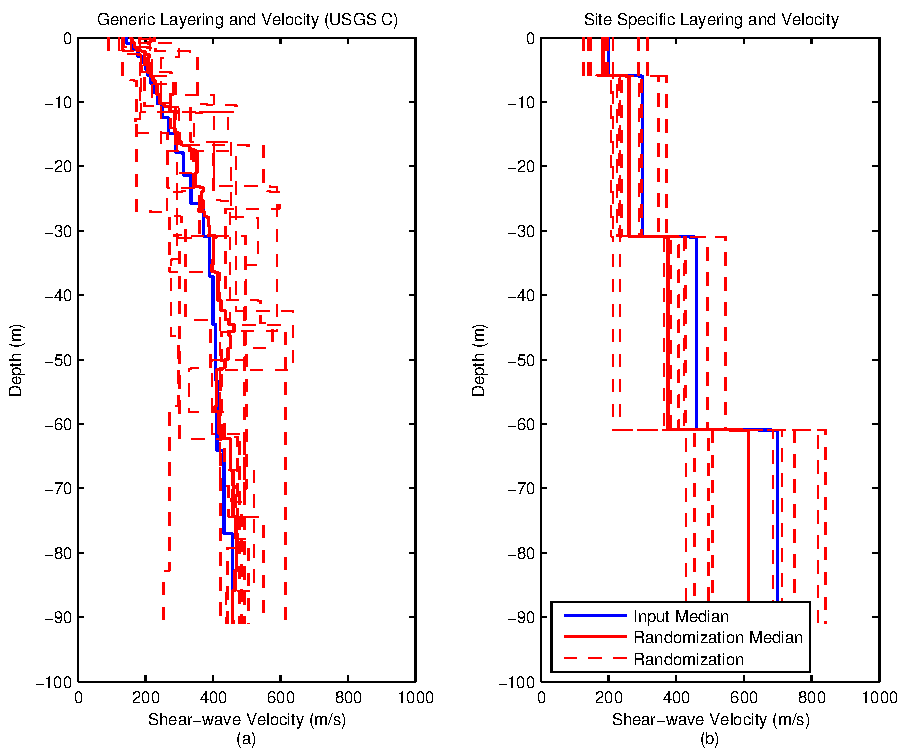
\includegraphics[width=\linewidth]{figures/rand/profile.pdf}
  \end{center}
  \caption{Ten generated shear-wave velocity ($v_s$) profiles for a USGS C site class. (a) Using
  generic layering and median $v_s$, (b) using user defined layering and median $v_s$.}
  \label{fig:rand:vsProfile}
\end{figure}
\clearpage

\subsection{Depth to Bedrock Model}
\ldots
%FIXME finish this section


\subsection{Non-Linear Soil Properties Model} 
The \citet{darendeli:01} empirical model for nonlinear soil properties ($G/G_{max}$ and $D$) was
previously discussed in Section~\ref{ch:siteResponse:dynprops}.  The \citet{darendeli:01} empirical
model assumes the variation of the properties is normal in distribution.  The standard deviation of
the $G/G_{max}$ and the $D$ varies with the magnitude of the property and is calculated with
equations (\ref{eq:sigmaShear}) and (\ref{eq:sigmaDamping}), respectively.  Because the variation of
the properties are modeled with a normal distribution is continuous from $-\infty$ to $+\infty$, the
generated values of the shear-modulus reduction or damping ratio may fall below zero.  The most
likely location for the negative values occurs when the mean value is small, which occurs at large
strains for the $G/G_{max}$ and at low strains for $D$.  Negative values for either $G/G_{max}$ or
$D$ are not physically possible, therefore the normal distributions need to be truncated.  To
correct for this problem, minimum values for $G/G_{max}$ and $D$ are defined as 0.05 and 0.1\%,
respectively.  These values were chosen as they represent appropriate minimum values.  The influence
of the minimum values on the site response results will be minimal because the truncation occurs
only at the extremes of the strain range.

The $G/G_{max}$ and $D$ curves are not independent of each other.  Consider a soil that behaves
more linearly, that is to say the $G/G_{max}$ is higher than the median $G/G_{max}$.  During a
loading cycle, the area inside the hysteresis would be smaller which is indicative of less damping
within the system.  As the linearity of the system increases, the damping decreases.  To capture
this effect, the soil properties are assumed to have a negative correlation with the default value
set at -0.5 (i.e.  $\rho=-0.5$).  Using a correlation coefficient of -0.5, the nonlinear properties
of sand (PI=0, OCR=0) at a confining pressure of 1 atm were generated 10 times, shown in
Figure~\ref{fig:rand:nlProps}.  Three of the realizations result in large shear modulus reduction
curve relative to the mean.  Because of the negative correlation, the relative high shear modulus
reduction corresponds to a relative low damping ratio.

% FIXME update figure to reflect actual behavior of program
\begin{figure}[tp]
  \begin{center}
	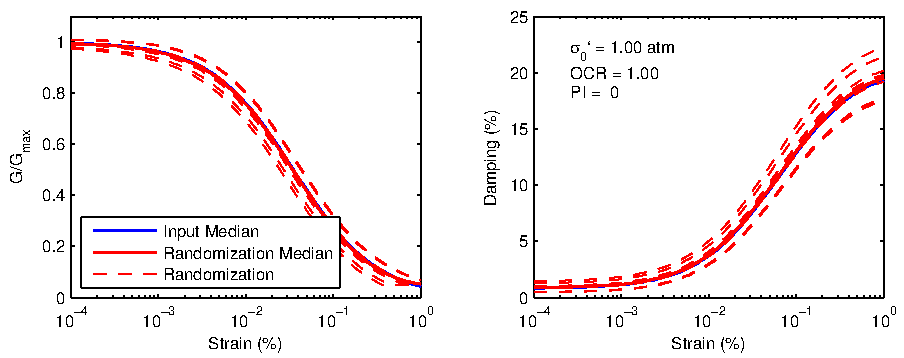
\includegraphics[width=\linewidth]{figures/rand/nlProps.pdf}
  \end{center}
  \caption{Generated nonlinear properties assuming perfect negative correlation.}
  \label{fig:rand:nlProps}
\end{figure}

\chapter{Using Strata}
Strata is introduced through two examples that demonstrates the organization and most of the
features found in Strata. Before these two examples some particular differences between Strata and
other site response programs are introduced. 

To someone that is used to working with text input files, operating Strata will seem a little
foreign.  With the exception of acceleration time-series, all of the input to Strata is
entered via the keyboard, or through copying and pasting from spreadsheets.  The input file is not
saved in the typical text format, instead a binary format is used that is only readable by Strata.
Furthermore, when the calculation is complete no output text files are produced.  Instead, the
output can be directly view with Strata and saved, once again to a binary format.  There is the
option for the data to be exported to text files that can then be opened with a variety of
applications.

\section{Strata Particulars}
\subsection{Auto-Discretization of Layers}
One of the biggest differences between Strata and other site response analysis programs is the fact
that the sublayers used in the calculation portion of the analysis are not defined by the user.
Instead, the user defines a velocity layer that is then subdivided into sublayers by Strata.  This
fundamental difference exists because Strata allows for the layering and shear-wave velocity to vary
(see Section~\ref{ch:var:models:layering} and therefore the required thickness of the sublayers
changes.

The maximum thickness ($h_\text{max}$) of the sublayers of $i$-th velocity layer is take as a
fraction of the minimum wavelength to be captured by the analysis:
\begin{equation}
	h_{\text{max},i} = \lambda_\text{frac} \cdot \lambda_\text{min} = \lambda_\text{frac} \cdot
	\frac{v_{s,i}}{f_\text{max}}
\end{equation}
where $\lambda_{\text{frac}}$ is the wavelength fraction which typically varies between $1/10$ and
$1/5$ (anything greater than $1/3$ is not recommended), $f_{\text{max}}$ is the maximum frequency of
engineering interest which is typically around 20 Hz, and $V_{s,i}$ is the shear-wave velocity of
the $i$-th layer.  The actual thickness of the sublayers is less than the maximum thickness such
that the velocity layer height divided by the sub-layer thickness is a whole number.  These
parameters are defined on the \texttt{General Settings} tab.  To prevent the layers from being
auto-discretized the wavelength fraction can be increased and the thickness velocity layers defined
in the \texttt{Soil Profile} tab can be reduced to an appropriate level.

In other site response programs, the location of the input motion or the location of
requested output (e.g., acceleration-time history) is generally referenced by a sublayer index.
However, because the sublayers are computed in Strata (and may change for
each realization), the location is defined in terms of the depth within the soil profile
or at the top of the bedrock.  When the location is specified as \texttt{Bedrock} then the actual depth
of the location will change if the depth of the bedrock changes.  The location is specified with a
drop down list shown in Figure~\ref{fig:strata:locationSlection} where the user can specify the
depth as \texttt{Bedrock} (Figure~\ref{fig:strata:locationSlection}a) or a fixed depth
(Figure~\ref{fig:strata:allRowsButton}c).

\begin{figure}[htb]
  \begin{center}
	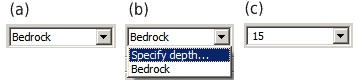
\includegraphics[scale=0.65]{figures/strata/locationSelection.png}
  \end{center}
  \caption[Strata location selection]{Location selection: (a) top of bedrock, (b) switching to a
  fixed depth, and (c) fixed depth of 15.}
  \label{fig:strata:locationSlection}
\end{figure}

\subsection{Interaction with Tables}
For the majority of Strata, the input behaves as you would expect.  The one exception may come when
editing tables. Table cells are selected with one click.  Once a cell is selected, the cell can be
edited by typing.  A cell's edit mode can be directly entered by double clicking on the cell.  In
some case double clicking on a cell will produce a widget to aid specifying input to the cell.

All tables used in Strata are dynamic meaning the number of rows can be changed. Rows are added to
the bottom on the list with the \emph{Add} button.  The \emph{Insert} and \emph{Remove} buttons are
disabled until once a complete row has been selected, which is most easily achieved by clicking on
the number next to the row of interest.  Multiple continuous rows can be selected by pressing the
\emph{shift} key while selecting the rows.  After rows have been selected: \texttt{Add} will add the
same number of rows to the end of the table, \texttt{Insert} will insert the same number of rows to
prior to the currently selected rows, and \texttt{Remove} will remove the selected rows.  All rows
in the table can be selected by click on the button in the upper right portion of the table as shown
in Figure~\ref{fig:strata:allRowsButton}. Some table has cells that can not be edited and have a
light gray background.  An example of these cells is in the \emph{Velocity Layers} table (shown
Figure~\ref{fig:strata:allRowsButton}).

\begin{sidewaysfigure}[tbp]
  \begin{center}
	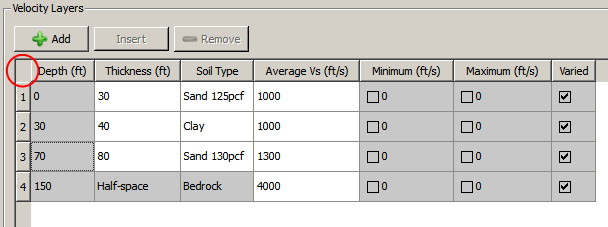
\includegraphics[scale=0.65]{figures/strata/allRowsButton.png}
  \end{center}
  \caption{By clicking on the button circled in red all rows in the table are selected.}
  \label{fig:strata:allRowsButton}
\end{sidewaysfigure}

Data can copied from spreadsheets and be pasted into tables by:
\begin{enumerate}
  \item Pressing \texttt{Ctrl+v}, 
  \item Clicking on the table, and then selecting \texttt{Paste} from the \texttt{Edit} menu, or
  \item Right clicking on the table and selecting paste.
\end{enumerate}
The table will automatically increase the numbers of rows to accommodate the size of the pasted
data.

\subsection{Non-Linear Curves}
The nonlinear (shear-modulus reduction and damping) curves can be specified through three
different methods in Strata: (1) fixed models that are present by default and cannot be removed, (2)
user defined curves that can be used across projects, and (3) temporary models that only exist for
the project.

\subsubsection{Fixed Non-Linear Models}

The following shear-modulus reduction models are included by default:
\begin{itemize}
  \item \citet{darendeli:01}
  \item \citet{iwasaki:76} -- 0.25 and 1.0 atm
  \item \citet{seed:70} -- Mean and Upper
  \item \citet{vucetic:91} -- PI = 0, 15, 50, 100, and 200
\end{itemize}
and the following damping curves are included by default:
\begin{itemize}
  \item \citet{darendeli:01}
  \item \citet{seed:70} -- Lower and Mean
  \item \citet{vucetic:91} -- PI = 0, 15, 50, 100, and 200
\end{itemize}

\subsubsection{User Defined Models}
Non-linear curve models can be defined for use across multiple projects by adding models to the
library.  The nonlinear property manager is opened by selecting \texttt{Add/Remove Non-Linear
Property Curves} from the \texttt{Tools} menu.  Using the dialog
(Figure~\ref{fig:strata:nonLinearCurveManager}), a new model can be defined by following these
steps:
\begin{enumerate}
  \item Click the \texttt{Add} button to add a new curve to with the normalized shear-modulus
	reduction or damping models list.
  \item Rename the model from ``Untitled`` to something meaningful.
  \item Add the data points to the curve.
\end{enumerate}
A curve can be removed by selecting the curve and then clicking on the \texttt{Remove} button.
Models defined in this manner will be added to the \texttt{nonLinearCurves.strd} file found in the
Strata installation folder.

\begin{figure}[p]
  \begin{center}
	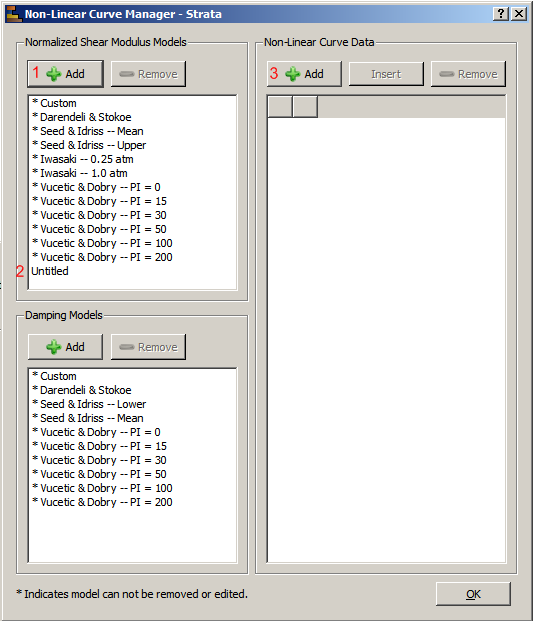
\includegraphics[width=\linewidth]{figures/strata/nonLinearPropertyManager.png}
  \end{center}
  \caption{The nonlinear curve manager.}
  \label{fig:strata:nonLinearCurveManager}
\end{figure}

\subsubsection{Temporary Models}
If you want to define a curve without adding it to the library of models, simply select
\texttt{Custom} from the drop-down list.  Changing to the \texttt{Custom} model does not clear the
previous models data which allows for a model to be modified.

\subsection{Recorded Motion Dialog}\label{ch:strata:particulars:motionDialog}
The \texttt{Recorded Motion Dialog} is used to load a recorded motion into Strata and appears when
the \texttt{Add} button is clicked in the \texttt{Record Motion(s)} table.  The dialog, shown in
Figure~\ref{fig:strata:recordedMotionDialog} allows the user to load a variety of motions in most
formats using the following steps:
\begin{enumerate}
  \item Click on the \texttt{File...} button and select the acceleration time series file.  If the
	file is from the NGA database, then the remainder of the form will be automatically completed as
	shown in Figure~\ref{fig:strata:recordedMotionDialogExample}.  Regardless of the file type, the
	file is read and loaded into the preview area.
  \item The remaining fields need to be filled to reflect the information in the file.  Information is
	required for all fields except for the \texttt{Description} field.  Fields can be
	completed by either typing values in, or selecting from the file preview and dragging the selected
	text into the field. The \texttt{Start line} and \texttt{Stop line} control which lines in the file
	contain the data.  A zero value for the \texttt{Stop line} will result in the data being read until
	the end of the file.  The file preview can be colored by clicking on the \texttt{Refresh} button.
	The colors have the following meanings:
	\begin{description}
	  \item[green] text found prior to the acceleration-time series data (ignored).
	  \item[blue] acceleration-time series data
	  \item[red] text after the time series data (ignored).
	\end{description}
	An example of the colored data is shown in Figure~\ref{fig:strata:recordedMotionDialogExample}.
  \item The scale factor can be selected at this time or after the motion has been loaded.  \emph{The scale
	factor should result in the motion being in units of gravity}.  After the motion has been loaded,
	the scale factor can also be adjusted by setting the peak-ground acceleration.
  \item After the form has been completed, the time-series can be viewed by clicking on the
	\texttt{Plot} button.
  \item Click \texttt{OK} to finish loading the file.
\end{enumerate} 

\begin{sidewaysfigure}[tpb]
  \begin{center}
	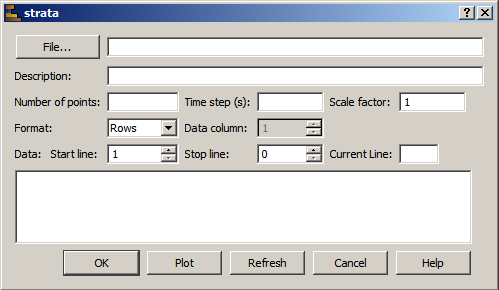
\includegraphics[scale=0.65]{figures/strata/recordedMotionDialog.png}
  \end{center}
  \caption{The initial view of the \texttt{Recorded Motion Dialog}.}
  \label{fig:strata:recordedMotionDialog}
\end{sidewaysfigure}

\begin{sidewaysfigure}[tpb]
  \begin{center}
	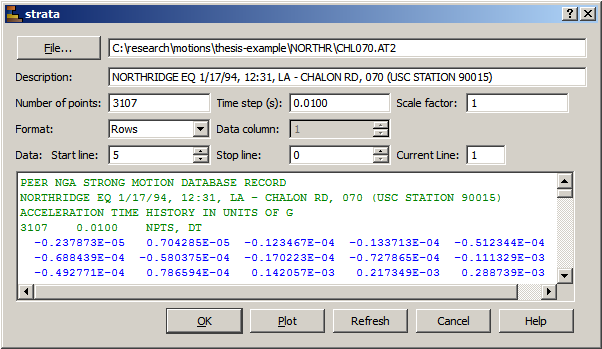
\includegraphics[scale=0.65]{figures/strata/recordedMotionDialogExample.png}
  \end{center}
  \caption{An example a completed \texttt{Recorded Motion Dialog}.}
  \label{fig:strata:recordedMotionDialogExample}
\end{sidewaysfigure}

\clearpage
\subsection{Output Widget}\label{ch:strata:particulars:outputWidget}
Once the site response calculation has been completed the view will change to the \texttt{Output
Widget}.  The \texttt{Output Widget} is also selected if a Strata output file is opened, or by
selecting \texttt{Output View} from the \texttt{Window} menu.  

Strata does not output any data files automatically.   The data can also be exported by selecting
\texttt{Export\dots} from the \texttt{File} menu.  The exported data file is in a comma-separated
values (CSV) format that can be easily opened with Excel or other spreadsheet program.  All data
(even disabled results) are included in the files.

Each result is characterized by a site realization and a motion.  If the data is enabled, the check
box with be checked, otherwise it is considered disabled.  Results that are enabled will be included
when the statistics are calculated. At the bottom of the table there are two buttons that allow all
motions or sites related to the currently selected result to be enabled or disabled.  In the example
(Figure~\ref{fig:strata:outputWidget}), both the site and motion are enabled.  Whenever the status
of a result is changed (e.g. from disabled to enabled) the \texttt{Recompute Statistics} button will
become enabled allowing the user to update the median and standard deviation.

The \texttt{Output Widget} shown in Figure~\ref{fig:strata:outputWidget} is used to
examine the results of a calculation.  In the figure, the output is acceleration response spectrum
computed at the surface for 20 motions and 20 different site profiles.  A individual result can be
selected by either clicking on the corresponding in the \texttt{Data Selection} table, or by
clicking on the result in the plot.  In both cases, the result is colored green if the result is
enabled, or red if the result is disabled.  After the status of a result has been changed, the
\texttt{Recomputed Statistics} button will become enabled indicating that the median and standard
deviation (shown on the plot in solid and dash blue lines, respectively) need to be updated.  

\begin{sidewaysfigure}[p]
  \begin{center}
	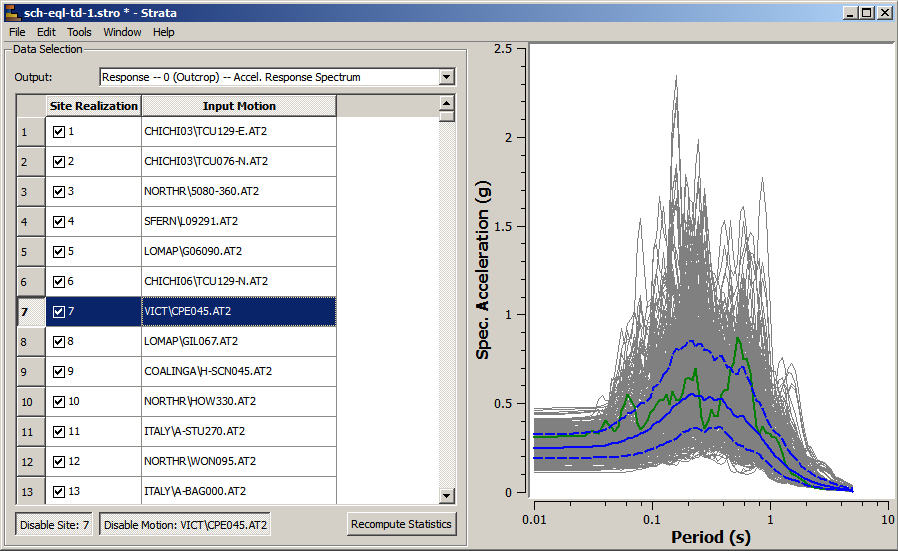
\includegraphics[scale=0.65]{figures/strata/outputWidget.png}
  \end{center}
  \caption{Using the Output view to examine the results of a calculation.}
  \label{fig:strata:outputWidget}
\end{sidewaysfigure}

The current plot can be printed by selecting \texttt{Print\dots} or \texttt{Print to PDF\dots} from
the \texttt{File} menu.  The current plot can also be copied by right clicking on the plot and
selecting \texttt{Copy}.

\section{Examples}
The following examples give a basic introduction to using Strata to perform equivalent linear site
response analysis.  The examples files are found within the \texttt{examples} folder in the
installation path.  The examples can be opened by either double clicking on their file, or selecting
them from the \texttt{Open\dots} item from the \texttt{File} menu.

All examples use the deep alluvium Sylmar County Hospital Parking Lot (SCH) site located in Southern
California for the site profile.  The soil types and velocity layering of the site was proposed by
\citet{chang:96}.  The soil properties are listed in Table~\ref{tab:strata:sylmar:soil} with a water
table at a depth of 46 meters. The nonlinear properties for each of the layers were computed using
the \citet{darendeli:01} empirical model with PI=0, OCR=1, and the confining pressures listed in
Table~\ref{tab:strata:sylmar:soil}.  The corresponding velocity profile is shown in
Figure~\ref{fig:strata:sylmar:vsProfile}. The time-averaged shear-wave velocity over the top 30
meters was computed as 273 m/s which classifies the site as a USGS site class C.

\begin{sidewaystable}
  \centering
  \begin{tabular}{cllccc}
	\hline\hline
	\textbf{Depth Range} (m) & \textbf{Soil Type} & \textbf{V$_\text{s}$} (m/s) &
	\textbf{$\gamma_\text{tot}$} (kN/m$^3$) & \textbf{$\sigma_v'$} (kPa) & \textbf{$\sigma_{m}'$} (atm) \\
	\hline
	0 to 6 & Alluvium (Sand) & 200 (150 to 230) & 18 & 54 & 0.36\\
	6 to 31 & Alluvium (Sand) & 300 (240 to 350) & 18 & 222 & 2.2 \\
	31 to 61 & Alluvium (Sand) & 460 (370 to 550) & 19 & 562 & 5.6 \\
	61 to 91 & Alluvium and Older & 700 (580 to 750) & 22 & 776 & 7.7 \\
	& Alluvium (Sand) \\
	91+ & Bedrock & 760 & 22 \\
	\hline\hline
  \end{tabular}
  \caption{Soil profile at the Sylmar County Hospital Parking Lot site~\citep{chang:96}. The mean
  effective stress ($\sigma_{m}'$) is computed assuming a $k_0$ of 1/2 and a water table depth of 46
  meters.}
  \label{tab:strata:sylmar:soil}
\end{sidewaystable}

\begin{figure}[tbp]
  \begin{center}
	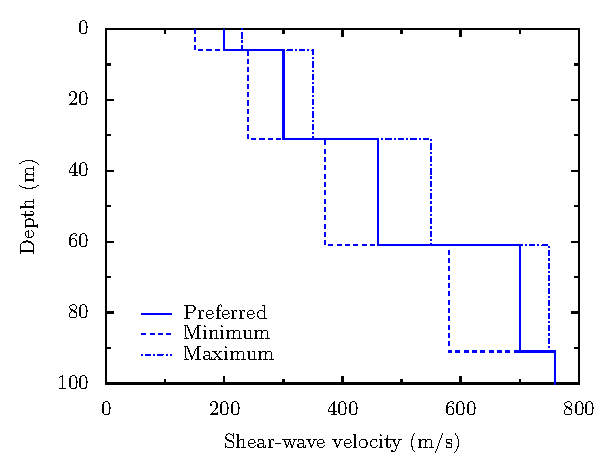
\includegraphics{figures/strata/sylmar-vs-profile}
  \end{center}
  \caption{The shear-wave velocity profile of the Sylmar County Hospital Parking Lot
  site~\citep{chang:96}.}
  \label{fig:strata:sylmar:vsProfile}
\end{figure}

\subsection{Example 1: Basic time domain}\label{ch:strata:example:1}
In the first example, the site response will be computed for the Sylmar County Hospital Parking Lot
site using seven different recorded motions.  This example can be opened from the
\texttt{example-1-td.stri} file in the \texttt{examples} directory.  Strata has the option of saving
the time-series data within the project file which is useful when the project files is transferred
to different computers.  For this example, the acceleration-times series are included in the project
file.  While the different tabs in the project can be accessed in any order, going from
left-to-right is preferred as information in one tab may depend on tabs to the left of it.

\subsubsection{Defining soil types}
A soil type is defined by a name, unit weight, an initial damping, shear-modulus reduction model,
damping model, and notes about the soil type.  The name is only used to identify the soil type, and
the notes are only present to type maintain sanity.  For soil types that use the
\citet{darendeli:01} model for either of nonlinear properties, addition properties required by the
empirical model must be defined.

For the site profile presented in Table~\ref{tab:strata:sylmar:soil}, four different soil types are
required.  Each soil type uses the \citet{darendeli:01} model for both the shear-modulus reduction
and damping, but the mean effective stress in the model changes.

\subsubsection{Defining soil profile}
The soil profile combines the shear-wave velocity profile and soil types together.  For each soil
layer in the profile, requires that a thickness, soil type, and shear-wave velocity must be
assigned.  The soil types are selected from a list of soil types defined in the \texttt{Soil Types}
tab.

\subsubsection{Defining the acceleration-time series}
The example provides seven acceleration-time series scaled to a target response spectrum and
standard deviation.  A motion is added by clicking on the \texttt{Add} button in the
\texttt{Recorded Motion(s)} table.  After clicking add a dialog will appear to assist in loading the
file, information on this dialog is presented in Section~\ref{ch:strata:particulars:motionDialog}.
Once the motion has been loaded, only the scale factors can be changed by either specifying a
peak-ground acceleration or a scale factor.  If the \texttt{Save motion data with the input file}
check box is checked, then the Strata input file will contain all of the information regarding the
time series.  This increases the size of the input file, but allows for a single file to contain all
required input.

\subsubsection{Defining the output}
There are generally four different types of output that can be computed by Strata:
\begin{description}
  \item[Response location output] involves the response at a given location (e.g. acceleration
	response spectrum or a time series).
  \item[Ratio output] involves the ratio of a response at two different location at a given location
	(e.g. transfer function or spectral ratio).
  \item[Profile] variation of a property with depth (e.g. maximum shear-strain).  The profiles are
	computed at particular depths because the layering of the model may change as a result of variation. 
  \item[Non-linear curves] the nonlinear curves.
\end{description}

Note: Only the information requested is stored.

\subsubsection{Computing}
After the project is fully defined, switch the \texttt{Compute} tab and click on the
\texttt{Compute} button.  Information regarding the calculation will be displayed in the window and
once the calculation is complete the view will switch to the output widget.  For more information
on using the output widget see Section~\ref{ch:strata:particulars:outputWidget}.  The input widget
can be selected by selected \texttt{Input View} from the \texttt{Window} menu, or by pressing
\texttt{F2}.

\subsection{Example 2: RVT and Site Variation}\label{ch:strata:example:2}
In the second example, the site response for the SCH site using random vibration theory and
variation of the shear-wave velocity profile. This example can be opened from the
\texttt{example-2-rvt.stri} file in the \texttt{examples} directory.  The site profile is exactly
the same as was used in the previous example.  There are only two changes that will be discussed:
the change from time domain to random vibration theory, and how to enable site variation.  Both of
these settings are enabled in the \texttt{General Settings} tab.
Figure~\ref{fig:strata:example:2:generalSettings} shows the proper settings for enabling RVT and
shear-wave velocity variation.

\begin{figure}[h]
  \begin{center}
	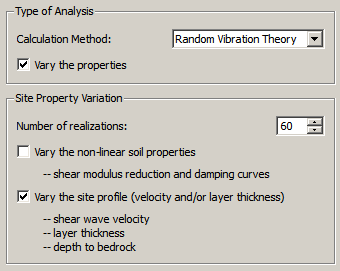
\includegraphics{figures/strata/example-2-generalSettings}
  \end{center}
  \caption{Settings to enable RVT site response and variation of the shear-wave velocity.}
  \label{fig:strata:example:2:generalSettings}
\end{figure}

\subsubsection{Varying the shear-wave velocity}
The parameters that control the shear-wave velocity variation are found on the \texttt{Soil Profile}
tab.  By enabling variation of the site profile a number of new columns will appear in the velocity
layers table, as well as a new group box containing a number of properties to vary.  In this
example, only the shear-wave velocity will be varied using the \texttt{USGS C} parameters for both
the standard deviation and correlation models.

\subsubsection{Defining an input acceleration response spectrum}
Random vibration theory allows for the input motion to be defined using either a Fourier amplitude
spectrum (FAS) or an acceleration response spectrum.  In this example, a response spectrum was computed
using \citet{abrahamson:97} empirical model for a magnitude 7.0 earthquake generated by a
strike-slip fault with a distance of 20 km.  The duration of the event was computed uses the
\citet{abrahamson:96} empirical relationship for the duration using an normalized Arias intensity of
0.75.  Whenever a response spectrum is used for input it is important to check that the resulting
FAS looks appropriate.  Strata allows the user to see both the data and the plots of the data prior
to the calculation.


\newpage
\bibliography{references}

\newpage
\printindex

\end{document}
